\documentclass{article}

\usepackage{graphicx}
\usepackage{caption}
\usepackage{subcaption}
\usepackage{float}
\usepackage{amsmath}
\usepackage{hyperref}


\title{COMP2020 Project 1: ALU - Project documentation}
\author{Nguyen Xuan Truong, V202300998}
\date{November 2024}
\begin{document}
\maketitle
\section{Overview}
\hspace*{2em}The ALU32-bit can perform a variety of arithmetic operations, including addition, subtraction, left shift, logical right shift, arithmetic right shift, equality check, inequality check, less than or equal to zero, greater than zero, AND, OR, XOR, and NOR. These operations are divided into four main blocks, each responsible for specific operations: the Add and Sub 32-bit block, the Shifter 32-bit block, the Comparator 32-bit block, and the Logical 32-bit block. The results of each block are then passed through a 32-bit OR gate. 

The following sections will explore each of the four main blocks and their respective subcomponents in detail.
\begin{center}
    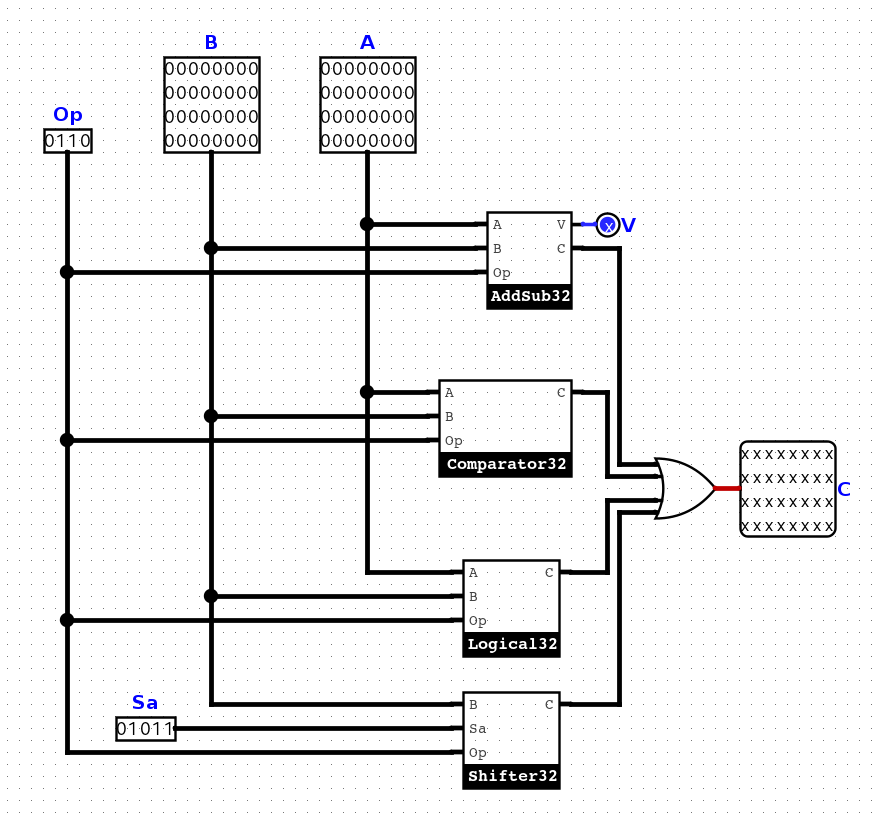
\includegraphics[width=0.8\textwidth]{images/Overview.png}
\end{center}
\captionof{figure}{ALU overview}

\section{Adder and Subtractor 32bit}
\hspace*{2em}The block adder and subtractor is constructed using only a 32-bit adder.This 32-bit adder is composed of various components, including a 1-bit adder, a 4-bit adder, a 4-bit adder with overflow handling, a 16-bit adder, and a 16-bit adder with overflow handling. The following sections will provide a detailed explanation of each subcomponent of the block adder and subtractor.
\subsection{Adder 1bit}
\begin{center}
    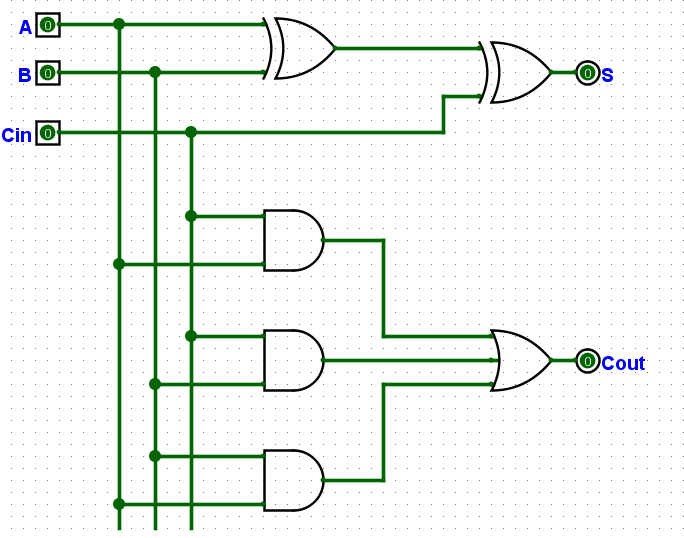
\includegraphics[width=1\textwidth]{images/Add1.png}
\end{center}
\captionof{figure}{1bit adder}
\hspace*{2em}This is the smallest unit of the 32-bit adder. It follows the basic truth table for addition with two 1-bit inputs, A and B, and a 1-bit carry-in. The output consists of a 1-bit sum (S) and a 1-bit carry-out.

\hspace*{2em}Total gate count of this block is 6 gates

\hspace{2em}The critical path of this block is 2
\begin{center}
\renewcommand{\arraystretch}{1.5} % Adjust row spacing
\begin{tabular}{|c|c|c|c|c|}
\hline
\textbf{A} & \textbf{B} & \textbf{C$_{in}$} & \textbf{C$_{out}$} & \textbf{S} \\
\hline
0 & 0 & 0 & 0 & 0 \\
\hline
0 & 0 & 1 & 0 & 1 \\
\hline
0 & 1 & 0 & 0 & 1 \\
\hline
0 & 1 & 1 & 1 & 0 \\
\hline
1 & 0 & 0 & 0 & 1 \\
\hline
1 & 0 & 1 & 1 & 0 \\
\hline
1 & 1 & 0 & 1 & 0 \\
\hline
1 & 1 & 1 & 1 & 1 \\
\hline
\end{tabular}   

\end{center}
\subsection{Adder 4bit}
\begin{center}
    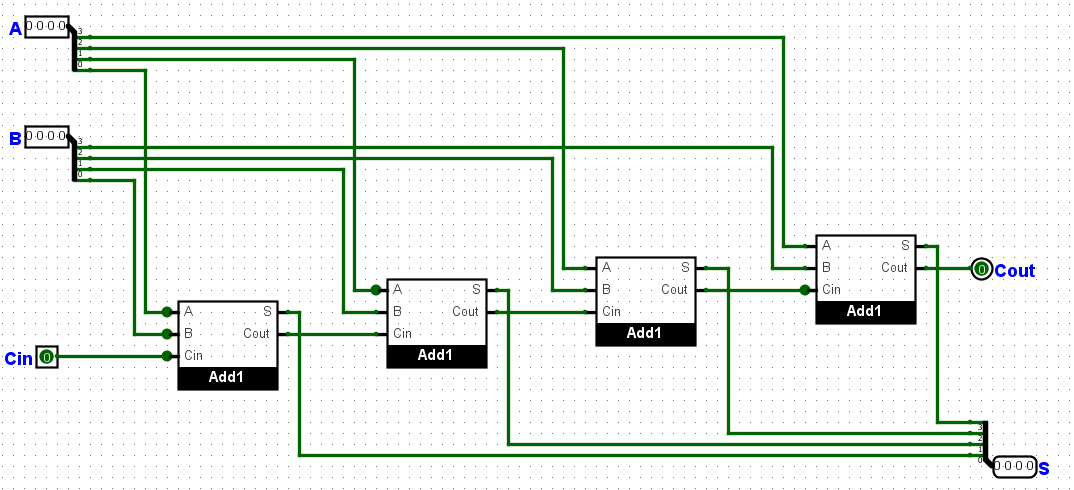
\includegraphics[width=1\textwidth]{images/Add4.png}
\end{center}
\captionof{figure}{4bit adder}
\hspace*{2em}The 4-bit adder consists of four 1-bit adders. The carry-in for each subsequent 1-bit adder block is the carry-out from the previous 1-bit adder. The inputs A and B are 4 bits wide. Starting from the least significant bit (rightmost) to the most significant bit (leftmost), each bit passes through its respective 1-bit adder block, producing the corresponding output bit. The carry-out of the final 1-bit adder is the carry-out of the entire 4-bit adder block.

\hspace*{2em}Each Add1 block has 6 gates counts. Then the total of gate counts of this block is 6 * 4 = 24

\hspace{2em}In this case each Add1 block got 2 critical path then the critical path of this block will got 2 * 4 = 8 critical path

\subsection{Adder 4bit overflow}
\begin{center}
    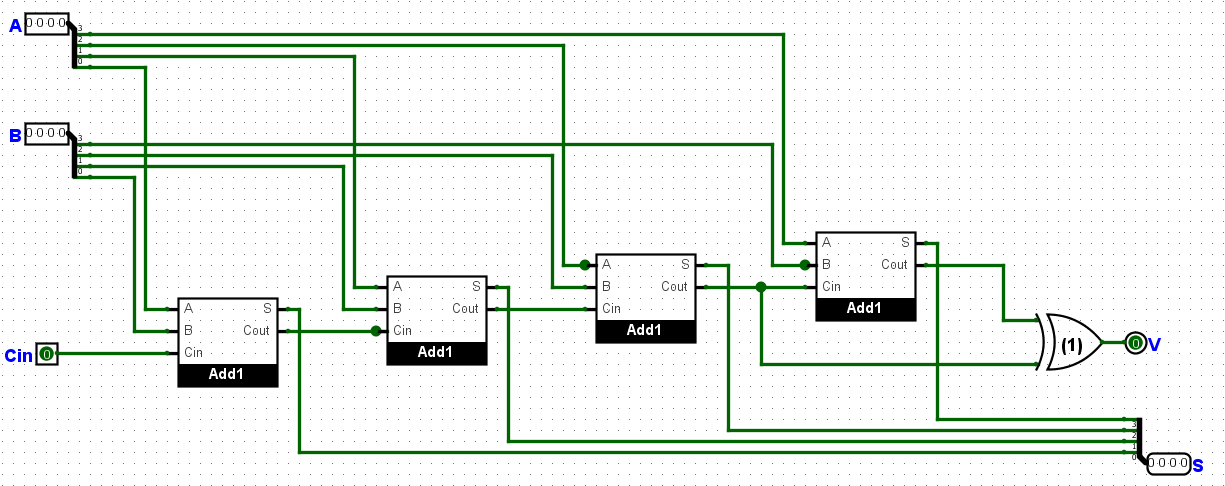
\includegraphics[width=1\textwidth]{images/Add4V.png}
\end{center}
\captionof{figure}{4bit adder with overflow}
\hspace*{2em}The 4-bit adder with overflow consists of four 1-bit adders and operates similarly to the regular 4-bit adder. The main difference is that the carry-in and carry-out of the last 1-bit adder block are XORed together (labeled as "XOR 1") to produce the overflow result.

\hspace{2em}Each Add1 block has 6 gates counts, with the last xor. Then the total of gate counts of this block is 6 * 4 + 1 = 25

\hspace{2em}In this case each Add1 block got 2 critical path then the critical path of this block 2 * 4 + 1 (from the last XOR gate) = 9
\subsection{Adder 16bit}
\begin{center}
    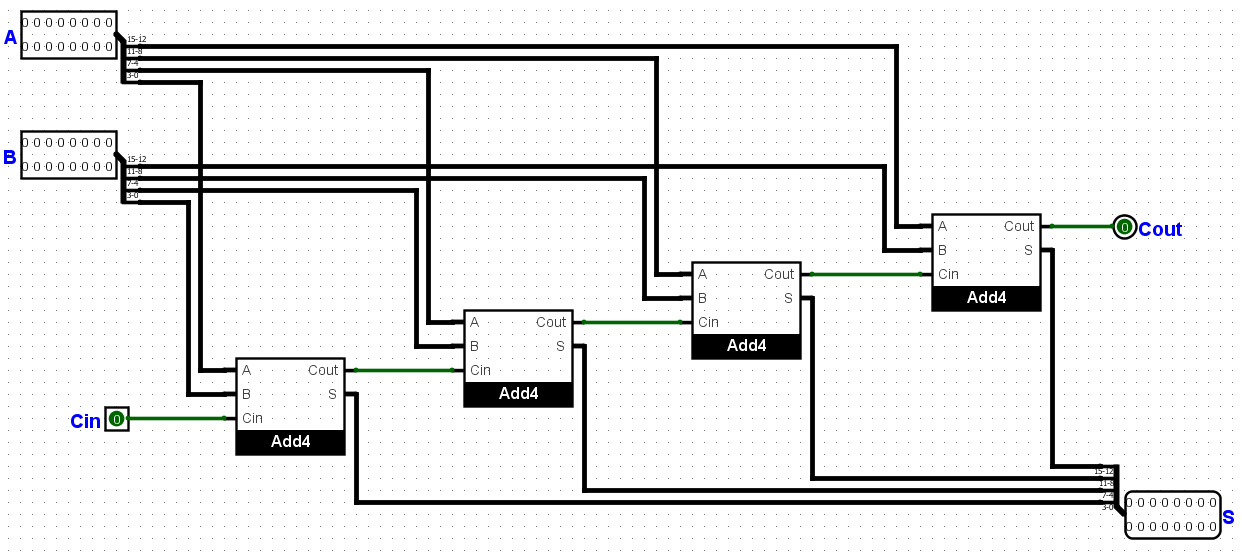
\includegraphics[width=1\textwidth]{images/Add16.png}
\end{center}
\captionof{figure}{16bit adder}
\hspace*{2em}The 16-bit adder operates similarly to a 4-bit adder but consists of four 4-bit adder blocks. The first block processes input bits 0 to 3, the second block handles bits 4 to 7, the third block processes bits 8 to 11, and the last block handles bits 12 to 15, with the outputs corresponding to their respective input ranges. The carry-out of the final 4-bit adder serves as the overall carry-out of the 16-bit adder.

\hspace{2em}Each Add4 block has 24 gates. Then the total of gate counts of this block is 24 * 4 = 96 gates

\hspace{2em}In this case each Add4 block got 8 critical path length then the critical path of this block 8 * 4 = 32
\subsection{Adder 16bit overflow}
\begin{center}
    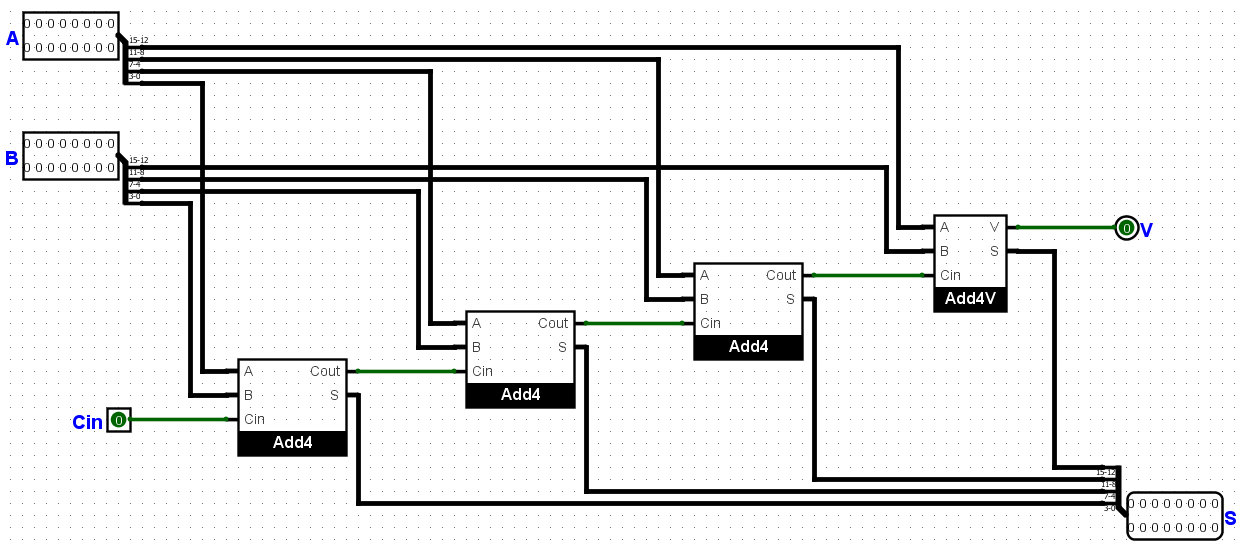
\includegraphics[width=1\textwidth]{images/Add16V.png}
\end{center}
\captionof{figure}{16bit adder with overflow}
\hspace*{2em} The 16-bit adder with overflow functions similarly to a regular 16-bit adder but consists of three standard 4-bit adders and one 4-bit adder with overflow. The final 4-bit adder provides the overflow value.

\hspace{2em}Each Add4 block has 24 gates and the last Add4V has 25 gates. Then the total of gate counts of this block is 24 * 3 + 25 = 97 gates

\hspace{2em}In this case each Add4 block got 2 critical path then the critical path of this block 2 * 4 + 1 (from the last XOR gate) = 9

\hspace{2em}In this case each Add4 block got 8 critical path length. The last Add4V got 9 critical path length then the critical path of this block 8 * 3 + 9 = 33
\subsection{Adder 32bit overflow}
\begin{center}
    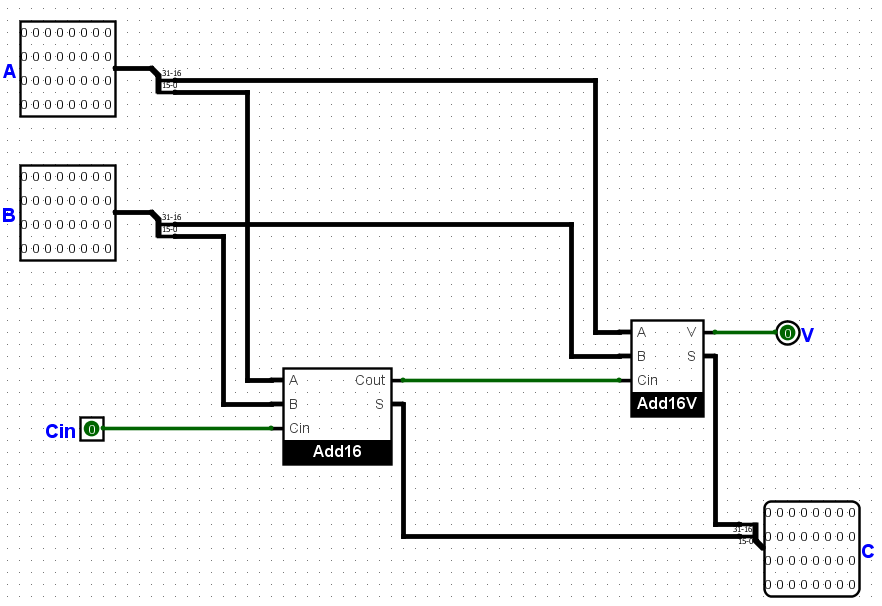
\includegraphics[width=1\textwidth]{images/Add32.png}
\end{center}
\captionof{figure}{32bit adder with overflow}
\hspace*{2em}The 32-bit adder with overflow consists of two blocks: a 16-bit adder and a 16-bit adder with overflow. The first block processes input bits 0 to 15, while the second block handles bits 16 to 31. The overflow result is determined by the 16-bit adder with overflow, and the carry-in is provided as input to the first 16-bit adder.

\hspace{2em}Add16 block has 96 gates and the Add16V has 97 gates. Then the total of gate counts of this block is 96 + 97 = 193 gates

\hspace{2em}In this case Add16 block got 32 critical path length. The last Add16V got 33 critical path length then the critical path of this block 32 + 33 = 65
\subsection{Operation bits}
\begin{center}
    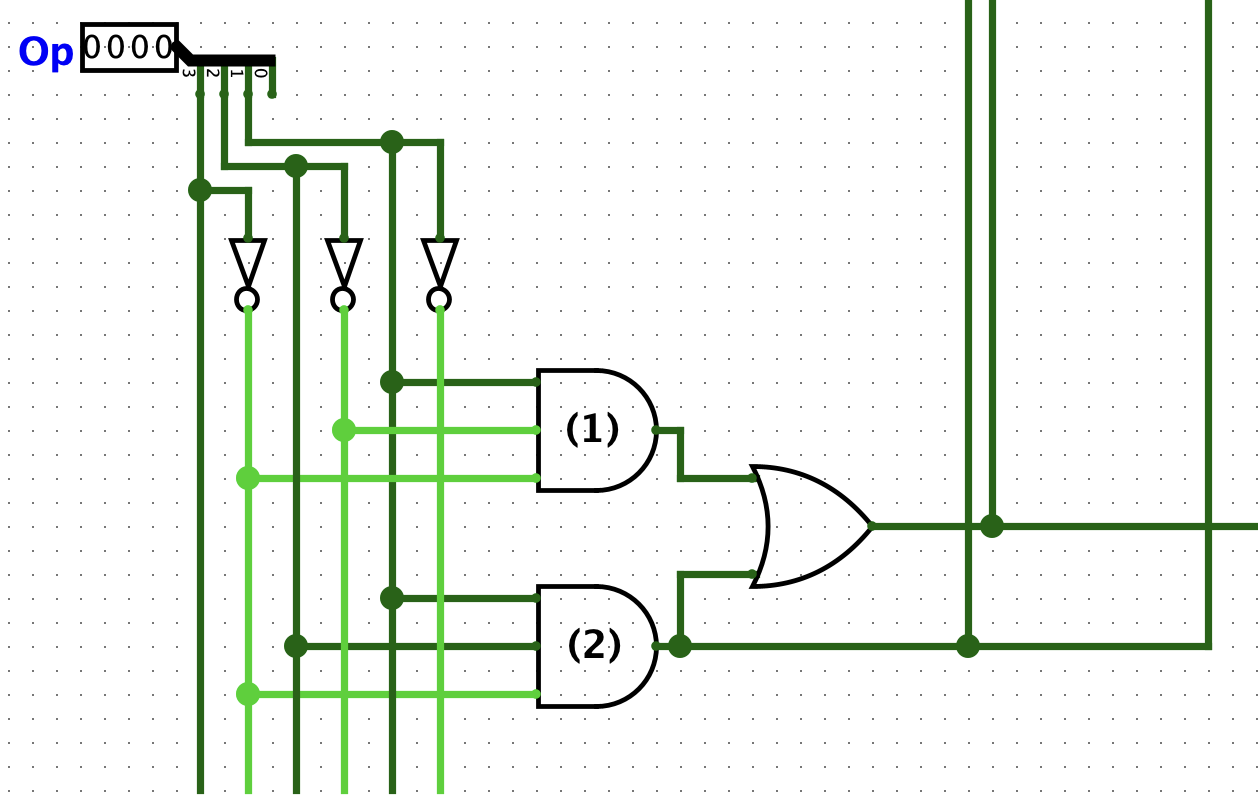
\includegraphics[width=0.7\textwidth]{images/AddSubSelectionsBits.png}
\end{center}
\captionof{figure}{Add and sub operation bits}
\hspace{2em}To design this operation bit circuit, we start by creating a truth table. From the truth table, we derive the Boolean equation using minterms and express it in the sum-of-products form.

\hspace{2em}This operations bits part got 3 gates.
\subsubsection{Truth table}
\begin{table}[h!]
\centering
\begin{tabular}{|c|c|c|c|c|c|c|c|}
\hline
\textbf{Name} & \textbf{Op} & \textbf{Op3} & \textbf{Op2} & \textbf{Op1} & \textbf{Op0} & \textbf{Enable bit} & \textbf{Output} \\ \hline
add           & 001x        & 0            & 0            & 1            & x            & 1                  & 0               \\ \hline
subtract      & 011x        & 0            & 1            & 1            & x            & 1                  & 1               \\ \hline
\end{tabular}
\end{table}
\subsubsection{Boolean equations}
The Boolean equations for the circuit are as follows:

\[
\text{Output} = \text{Op}_3' \cdot \text{Op}_2 \cdot \text{Op}_1
\]

\[
\text{EnableBit} = \text{Op}_3' \cdot \text{Op}_2 \cdot \text{Op}_1 + \text{Op}_3' \cdot \text{Op}_2' \cdot \text{Op}_1
\]
The output is defined by the AND term \(\text{Op}_3' \cdot \text{Op}_2 \cdot \text{Op}_1\) (the second AND block), which checks whether the operation is a subtract operation. The enable bit is formed by OR-ing two terms: \(\text{Op}_3' \cdot \text{Op}_2' \cdot \text{Op}_1\) (the first AND block) and \(\text{Op}_3' \cdot \text{Op}_2 \cdot \text{Op}_1\). This enable bit is then connected to the enable input of the multiplexer to ensure that the operation passed through this circuit corresponds to either add or subtract.


\subsection{Add/Sub Block}
\begin{center}
    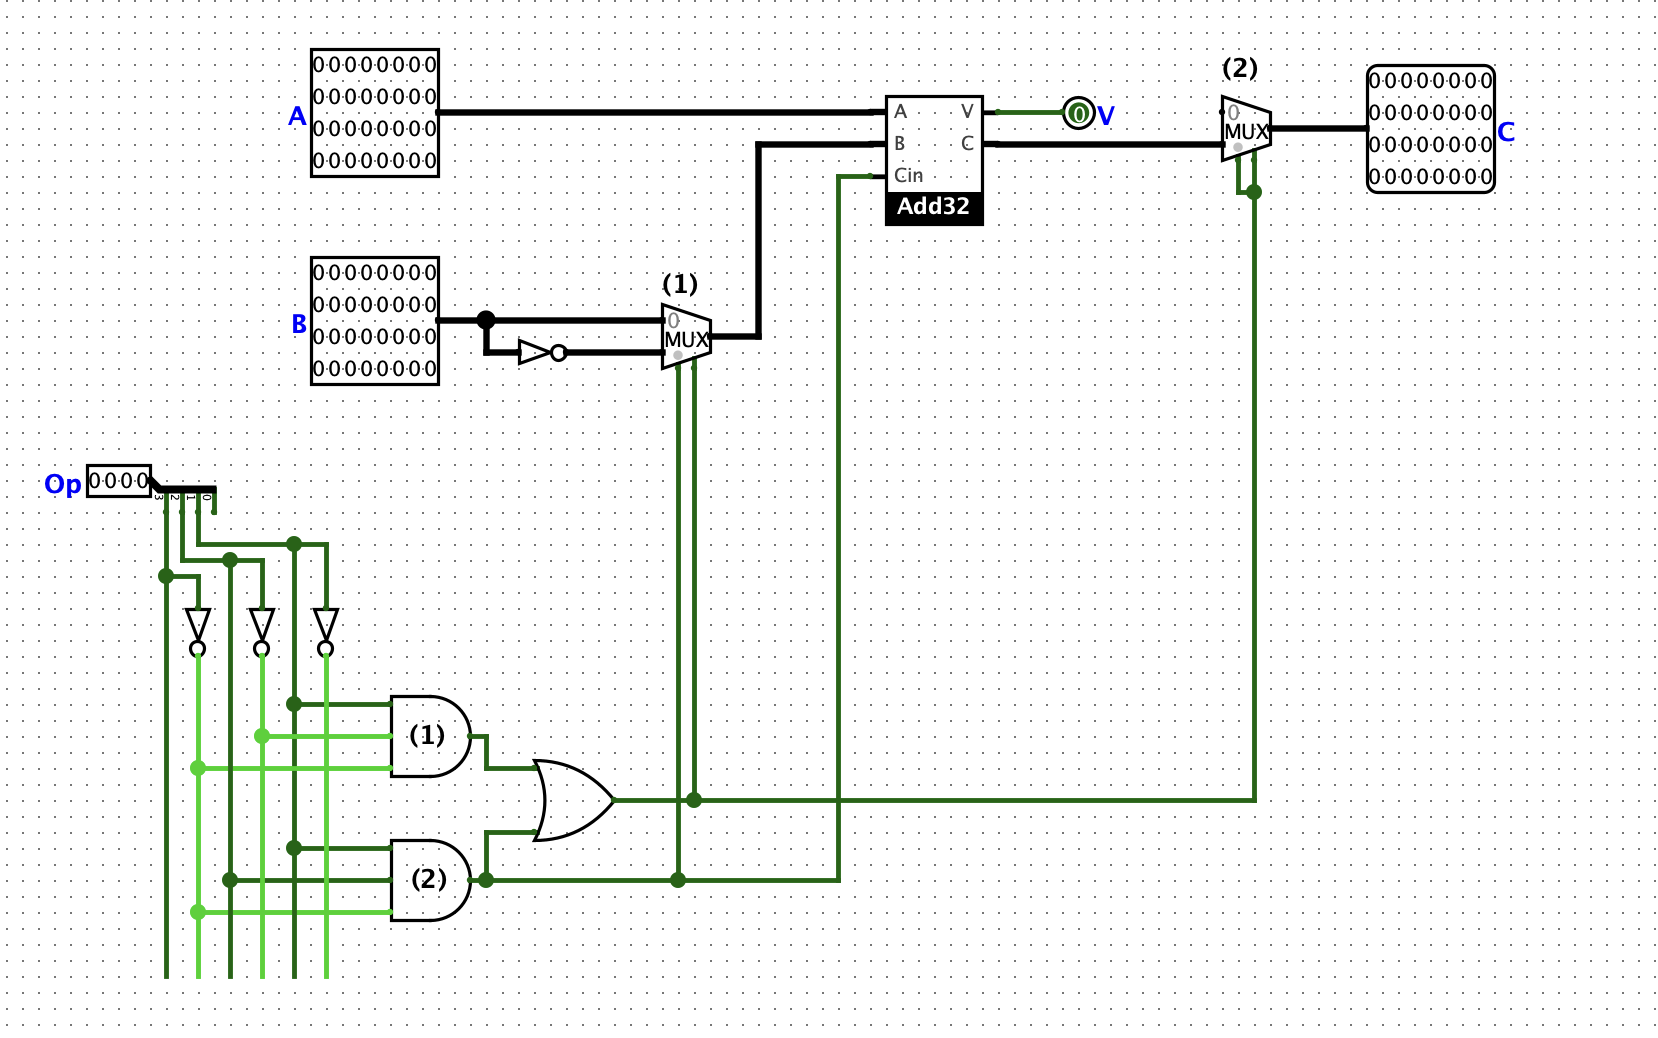
\includegraphics[width=1\textwidth]{images/AddSub32.png}
\end{center}
\captionof{figure}{Full 32bit adder and substractor block}
\hspace{2em} The \textbf{Add and Sub} block performs two main arithmetic operations: \textbf{Addition} and \textbf{Subtraction}. The design process is as follows:

\begin{enumerate}
    \item \textbf{Input B Selection:}  
    A multiplexer (\texttt{Mux1}) determines the value of input \( B \) for the \texttt{Add32} block:
    \begin{itemize}
        \item If the enable bit is \( 0 \), the value of input \( B \) is set to a 32-bit value of \( 0 \).
        \item If the enable bit is \( 1 \), the operation type is evaluated:
        \begin{itemize}
            \item For addition (\( op = \text{ADD} \)), \( B \) is directly selected.
            \item For subtraction (\( op = \text{SUBTRACT} \)), \( \overline{B} \) (bitwise negation of \( B \)) is selected.
        \end{itemize}
    \end{itemize}

    \item \textbf{Addition/Subtraction Logic:}  
    The \texttt{Add32} block takes inputs \( A \) and \( B \) from \texttt{Mux1}. The behavior depends on the operation:
    \begin{itemize}
        \item For addition, the carry-in is set to \( 0 \), and the result is \( A + B \).
        \item For subtraction, the carry-in is set to \( 1 \), as subtraction in two's complement is calculated as:
        \[
        A + \overline{B} + 1
        \]
    \end{itemize}

    \item \textbf{Output Selection:}  
    Another multiplexer (\texttt{Mux2}) determines the output:
    \begin{itemize}
        \item If the block is selected, the output is the result of \texttt{Add32}.
        \item If the block is not selected, the output is a 32-bit value of \( 0 \).
    \end{itemize}

    \item \textbf{Overflow:}  
    The overflow signal is directly taken from the overflow output of the \texttt{Add32} block.
\end{enumerate}

\hspace{2em}Two 2-to-1 MUX each got 32 * (2 + 1) = 96 gates then these two got 96 * 2 = 192 gates. The add32 block got 193 gates and the operations part got 3 gates. Then the total gate counts is 192 + 193 + 3 = 388 gates count

\hspace{2em}In this case 2 mux will got 2 critical path length each. Then the total critical path of this block 65 + 4 = 69
\section{Shifter 32bit}
\hspace*{2em}The block shifter is constructed using a 32-bit left shifter. This 32 bit left shifter is composed of various components, including 1-bit, 2-bit, 4-bit, 8-bit, and 16-bit left shifters. Additionally, the 32-bit shifter block utilizes two other components—the Most Significant Bit (MSB) and the Reverse32 bit—to perform left shifts, logical right shifts, and arithmetic right shifts.

\hspace*{2em}The following sections will provide a detailed explanation of each subcomponent of the block shifter.
\subsection{Left shifter 1bit}
\begin{center}
    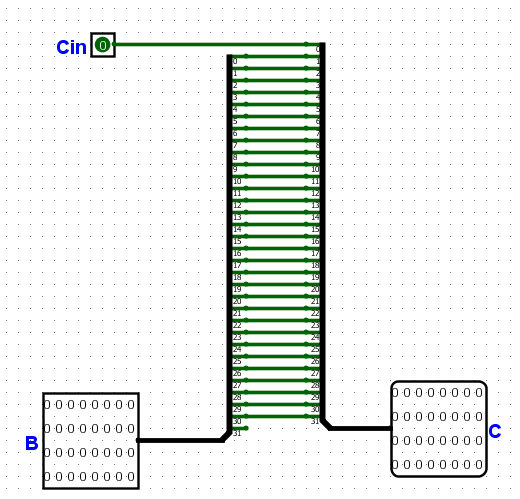
\includegraphics[width=0.5\textwidth]{images/LeftShift1.png}
\end{center}
\captionof{figure}{Shift left 1bit}
\hspace*{2em}To shift the input left by 1 bit, each output bit is connected to the input bit at its index minus one. As a result, the 32nd bit of the input is discarded, and the first output bit is set to the value of the carry-in.

\hspace{2em}This block got 0 gate count
\subsection{Left shifter higher bit}
\begin{figure}[H]
    \centering
    % First row
    \begin{subfigure}{0.45\textwidth}
        \centering
        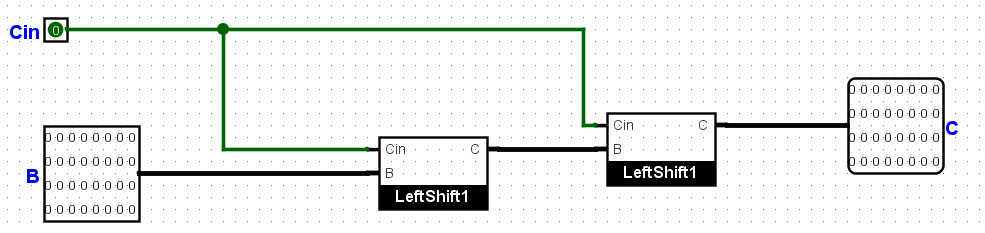
\includegraphics[width=\linewidth]{images/LeftShift2.png}
        \caption{Shift left 2bit}
        \label{fig:sub1}
    \end{subfigure}
    \hfill
    \begin{subfigure}{0.45\textwidth}
        \centering
        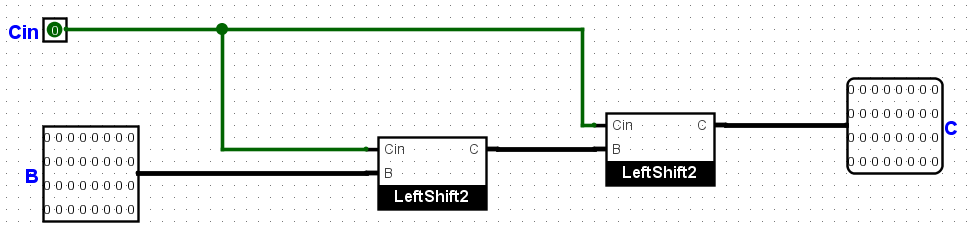
\includegraphics[width=\linewidth]{images/LeftShift4.png}
        \caption{Shift left 4bit}
        \label{fig:sub2}
    \end{subfigure}

    \vspace{0.5cm} % Space between rows

    % Second row
    \begin{subfigure}{0.45\textwidth}
        \centering
        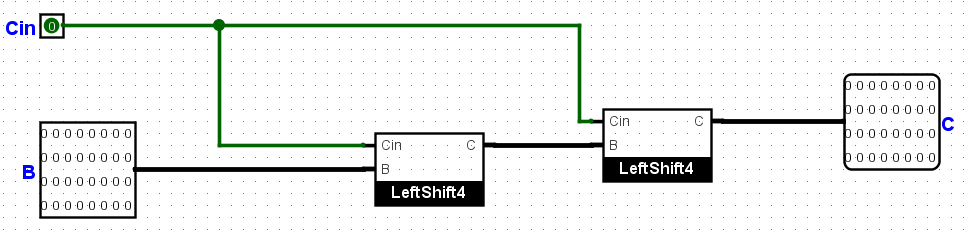
\includegraphics[width=\linewidth]{images/LeftShift8.png}
        \caption{Shift left 8bit}
        \label{fig:sub3}
    \end{subfigure}
    \hfill
    \begin{subfigure}{0.45\textwidth}
        \centering
        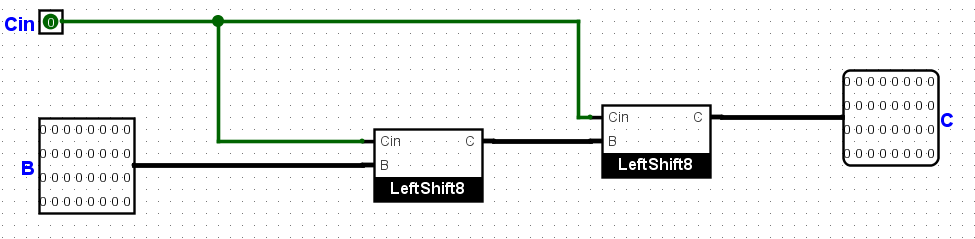
\includegraphics[width=\linewidth]{images/LeftShift16.png}
        \caption{Shift left 16bit}
        \label{fig:sub4}
    \end{subfigure}
    \caption{Group of left shift block 2bit, 4bit, 8bit and 16bit}
    \label{fig:group}
\end{figure}
\hspace*{2em}For higher-bit shifters, there are four main shifter blocks: 2-bit, 4-bit, 8-bit, and 16-bit. Each is constructed using two smaller-bit shifter blocks. The 2-bit shifter is created using two 1-bit left shifters, the 4-bit shifter uses two 2-bit left shifters, the 8-bit shifter uses two 4-bit left shifters, and the 16-bit shifter uses two 8-bit left shifters. The output of the first block serves as the input to the second block, and both blocks receive the carry-in signal.

\hspace{2em}These blocks all got 0 gate counts
\subsection{Left shift 32 bit}
\begin{center}
    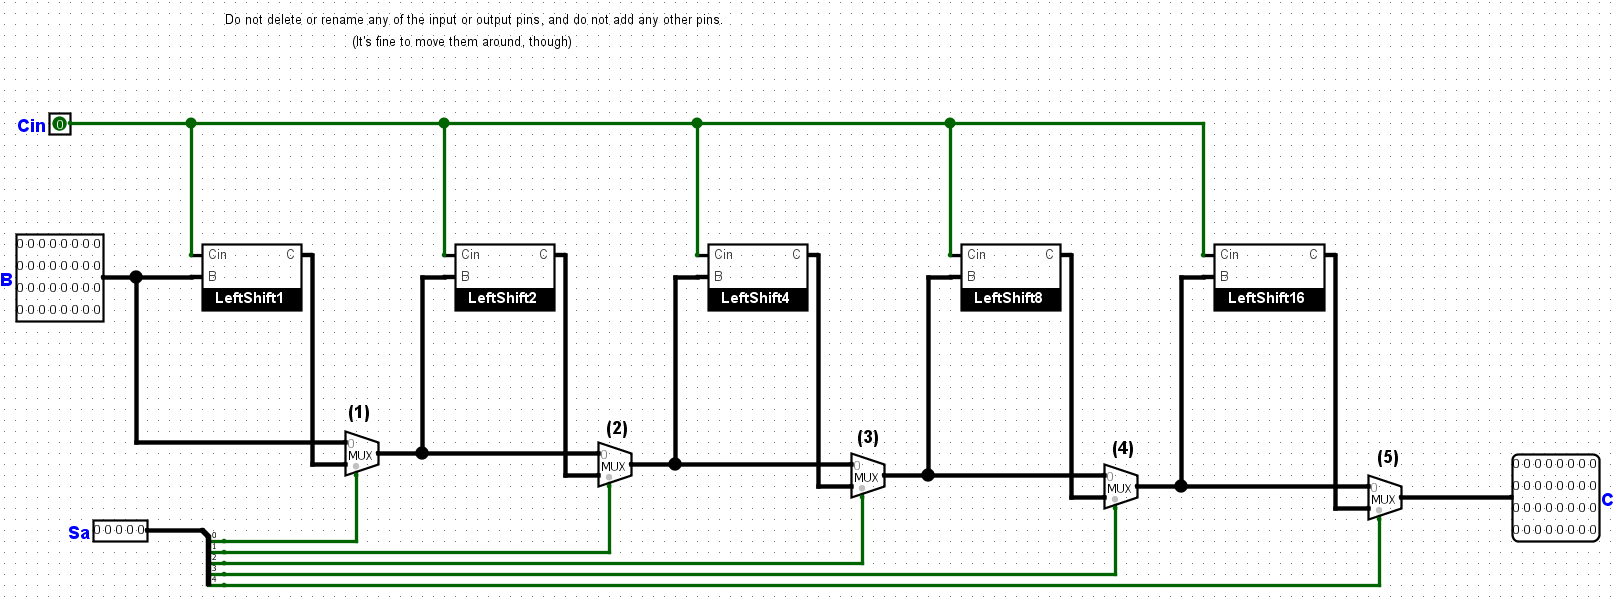
\includegraphics[width=1\textwidth]{images/LeftShift32.png}
\end{center}
\captionof{figure}{Shift left 32bit}
\hspace*{2em}The 32-bit left shifter performs flexible left shifts on a 32-bit input \( B \), based on a 5-bit shift magnitude \( S_a \) (ranging from 0 to 31) and a fill-in bit \( C_{in} \). It uses five sequential left-shift stages (shifting by 1, 2, 4, 8, and 16 bits) controlled by the corresponding bits of \( S_a \).
\hspace*{2em}Each stage passes its output through a multiplexer that selects either the shifted or unshifted result based on the control bit from \( S_a \). Cascading these stages enables the shifter to compute any shift as a sum of powers of 2 efficiently, minimizing latency while handling all valid shift values.

\hspace{2em}Each mux got 32 * (2 + 1) = 96 gates counts. Then this block got toal 96 * 5 = 480 gates counts

\hspace{2em}Only until this left shift 32 bit got 5 2-to-1 mux then the total critical path of this block is 2 * 5 = 10
\subsection{Reverse 32bit}
\begin{center}
    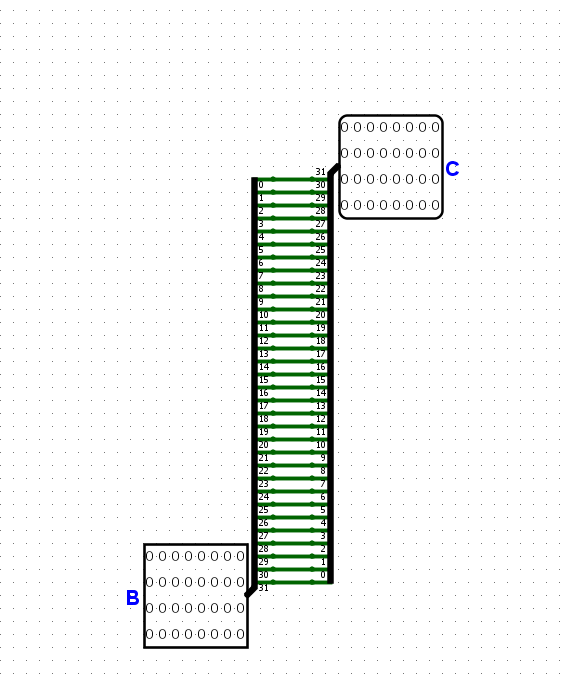
\includegraphics[width=1\textwidth]{images/Reverse32.png}
\end{center}
\captionof{figure}{Reverse 32bit}
\hspace{2em}This circuit reverses all the bits of \( A \). The bits of \( A \) are first split using a splitter, and then passed through another splitter that connects to output \( B \), with the bit order reversed.

\hspace{2em}This block got 0 gate counts
\subsection{Most significant bit}
\begin{center}
    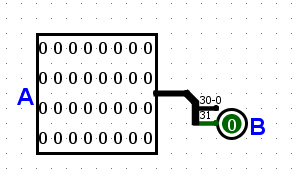
\includegraphics[width=0.5\textwidth]{images/MSB.png}
\end{center}
\captionof{figure}{Get most significant bit}
\hspace{2em} This circuit splits the 32-bit input, with bits 0 through 30 passed as the output, and the 31st bit is retained as the output.

\hspace{2em}This block got 0 gate counts
\subsection{Operation bits}
\begin{center}
    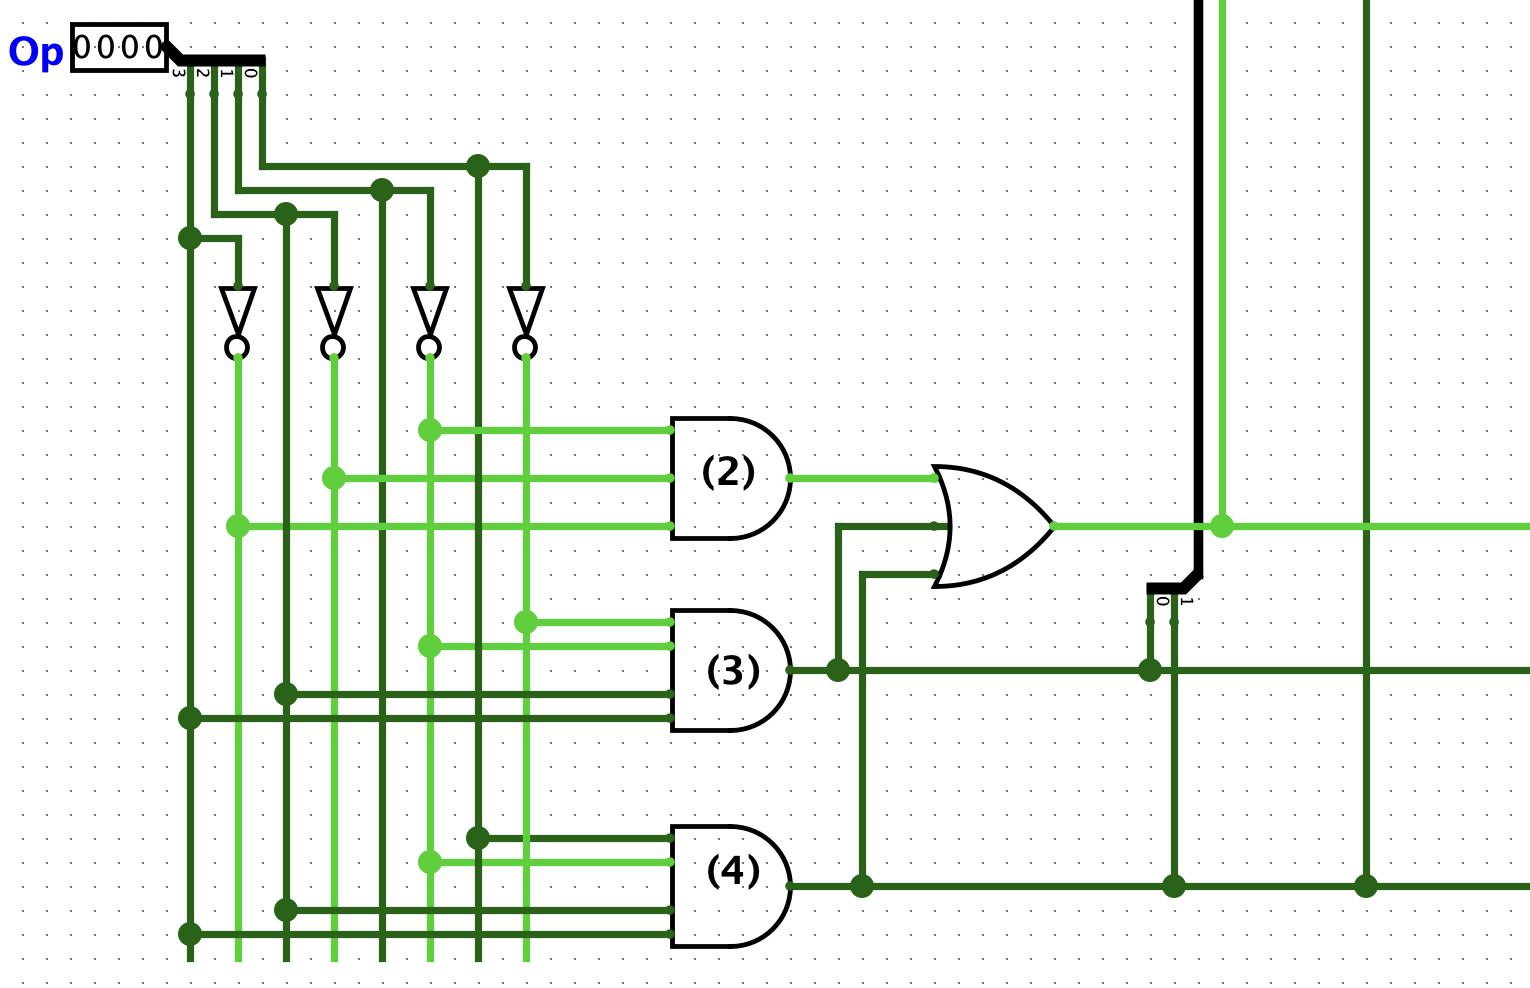
\includegraphics[width=0.8\textwidth]{images/ShifterSelectionBits.png}
\end{center}
\captionof{figure}{Shifter operation bits}
\hspace{2em}To design this operation bit circuit, we start by creating a truth table. From the truth table, we derive the Boolean equation using minterms and express it in the sum-of-products form.

\hspace{2em} This part got 4 gate counts
\subsubsection{Truth table}
\begin{table}[H]
\centering
\begin{tabular}{|c|c|c|c|c|c|c|c|c|c|}
\hline
Name & Op & Op3 & Op2 & Op1 & Op0 & Enable bit & Output 1 & Output 0 \\ \hline
shift left logical & 000x & 0 & 0 & 0 & x & 1 & 0 & 0 \\ \hline
shift right logical & 1100 & 1 & 1 & 0 & 0 & 1 & 0 & 1 \\ \hline
shift right arithmetic & 1101 & 1 & 1 & 0 & 1 & 1 & 1 & 0 \\ \hline
\end{tabular}
\end{table}

\subsubsection{Boolean equations}
The Boolean equations for the circuit are as follows:
\[
\text{Output}_0 = \text{Op}_3 \cdot \text{Op}_2 \cdot \text{Op}_1' \cdot \text{Op}_0'
\]
\[
\text{Output}_1 = \text{Op}_3 \cdot \text{Op}_2 \cdot \text{Op}_1' \cdot \text{Op}_0
\]
\[
\text{EnableBit} = \text{Op}_3' \cdot \text{Op}_2' \cdot \text{Op}_1' + \text{Op}_3 \cdot \text{Op}_2 \cdot \text{Op}_1' \cdot \text{Op}_0' + \text{Op}_3 \cdot \text{Op}_2 \cdot \text{Op}_1' \cdot \text{Op}_0
\]

The output is a 2-bit value defined by two bits. 

- The least significant bit is:

\[
\text{Op}_3 \cdot \text{Op}_2 \cdot \text{Op}_1' \cdot \text{Op}_0' \quad (\text{AND gate with label 3})
\]

- The most significant bit is:

\[
\text{Op}_3 \cdot \text{Op}_2 \cdot \text{Op}_1' \cdot \text{Op}_0 \quad (\text{AND gate with label 4})
\]

The output will identify the shifter:  
\[
\begin{array}{l}
00 \text{ for Shift Left Logical} \\
01 \text{ for Shift Right Logical} \\
10 \text{ for Shift Right Arithmetic}
\end{array}
\]

The enable bit will identify whether the shifter block can be run. The condition is ORed by 3 and \(\text{Op}_3' \cdot \text{Op}_2' \cdot \text{Op}_1'\) (the AND gate with label 2) with the AND gates labeled 3 and 4. This will connect with the enable bit of the multiplexer of the shifter block.

\subsection{Shifter Block}
\begin{center}
    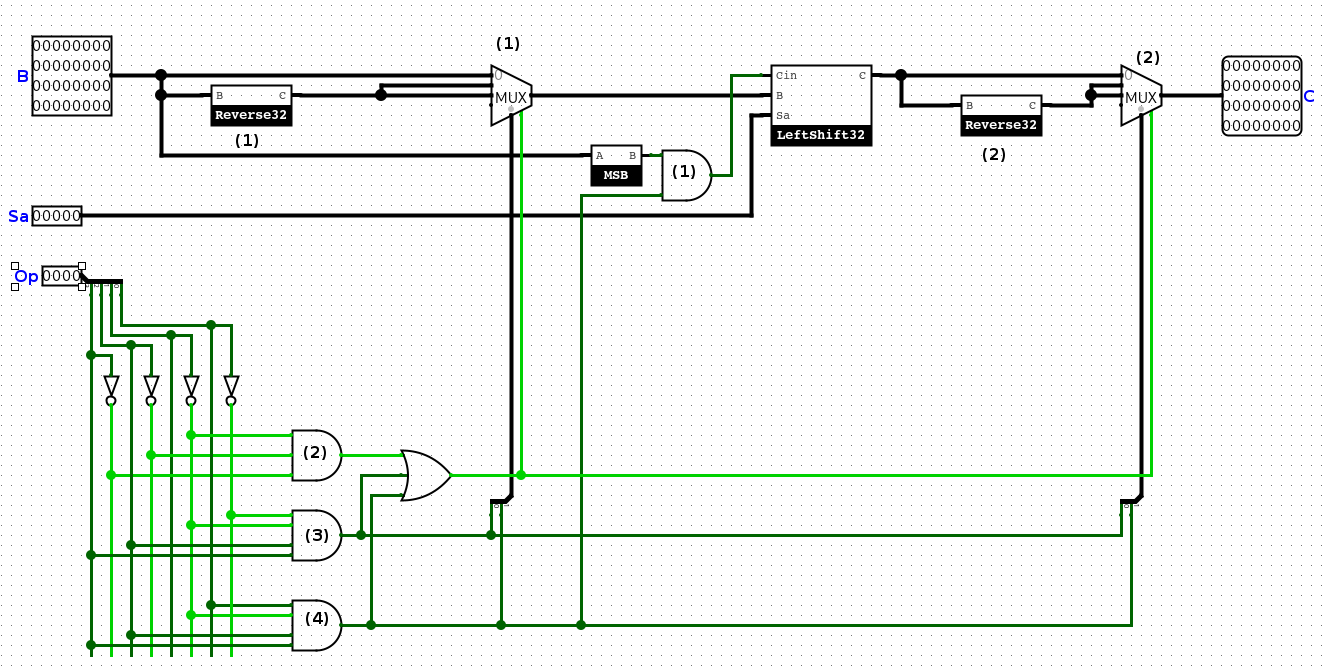
\includegraphics[width=1\textwidth]{images/Shifter32.png}
\end{center}
\captionof{figure}{Shifter 32bit block with shift left, shift right logical, and shift right arithmetic}

\hspace{2em}In the first stage of the block, the input \( B \) is processed as follows:

\begin{enumerate}
    \item \textbf{Reversal and Multiplexer (Mux1):}  
    The input \( B \) is first reversed (bitwise negation), resulting in four possible inputs for the multiplexer (\texttt{Mux1}):
    \begin{itemize}
        \item If the selection bits are \( 00 \) (left logical shift operation), the output \( B \) remains unchanged.
        \item If the selection bits are \( 01 \) or \( 10 \), the output \( B \) is the reversed \( B \).
    \end{itemize}

    \item \textbf{Left Shift Block (\texttt{LeftShift32}):}  
    The output \( B \) from \texttt{Mux1} is passed through the \texttt{LeftShift32} block, which performs the required shift. The shift amount is provided as an additional input.
    \begin{itemize}
        \item The carry-in for this block is determined by an AND gate (label 4) that evaluates the most significant bit (MSB) of the initial \( B \) and the opcode:
        \begin{itemize}
            \item If the operation is shift-right arithmetic and the MSB of the initial \( B \) is \( 1 \), the carry-in for the \texttt{LeftShift32} block is set to \( 1 \) (to extend the sign bit).
        \end{itemize}
    \end{itemize}

    \item \textbf{Final Reversal and Multiplexer (Mux2):}  
    The result of \texttt{LeftShift32} is reversed again before being passed to \texttt{Mux2}.
    \begin{itemize}
        \item \texttt{Mux2} uses the opcode to select the correct output for the block.
    \end{itemize}

    \item \textbf{Enable Bit Control:}  
    Both multiplexers (\texttt{Mux1} and \texttt{Mux2}) are controlled by an enable bit to determine if the output should be considered. If not enabled, the output is a 32-bit value of \( 0 \).
\end{enumerate}

\hspace{2em}Two 4-to-1 mux each got 32 * (4 + 1) = 160 gates count. One AND gates. The leftshift32 got 480 gate counts. Then the total gates counts of this block is 160 * 2 + 480 + 1 + 4 = 805 gates count.

\hspace{2em}The critical path of this block will be 2 + 10 + 2 = 14

\section{Comparator 32bit}
\hspace*{2em}The block comparator is composed of various components, including a bit extender (1 to 32), an equality checker, a zero-checker, a "less than or equal to zero" checker, and a "greater than zero" checker. This block can perform comparisons to determine whether \boldsymbol{A} and \boldsymbol{B} are equal, as well as check whether \boldsymbol{B} is greater than zero or less than or equal to zero.

The following sections will provide a detailed explanation of each subcomponent of the block comparator.
\begin{center}
    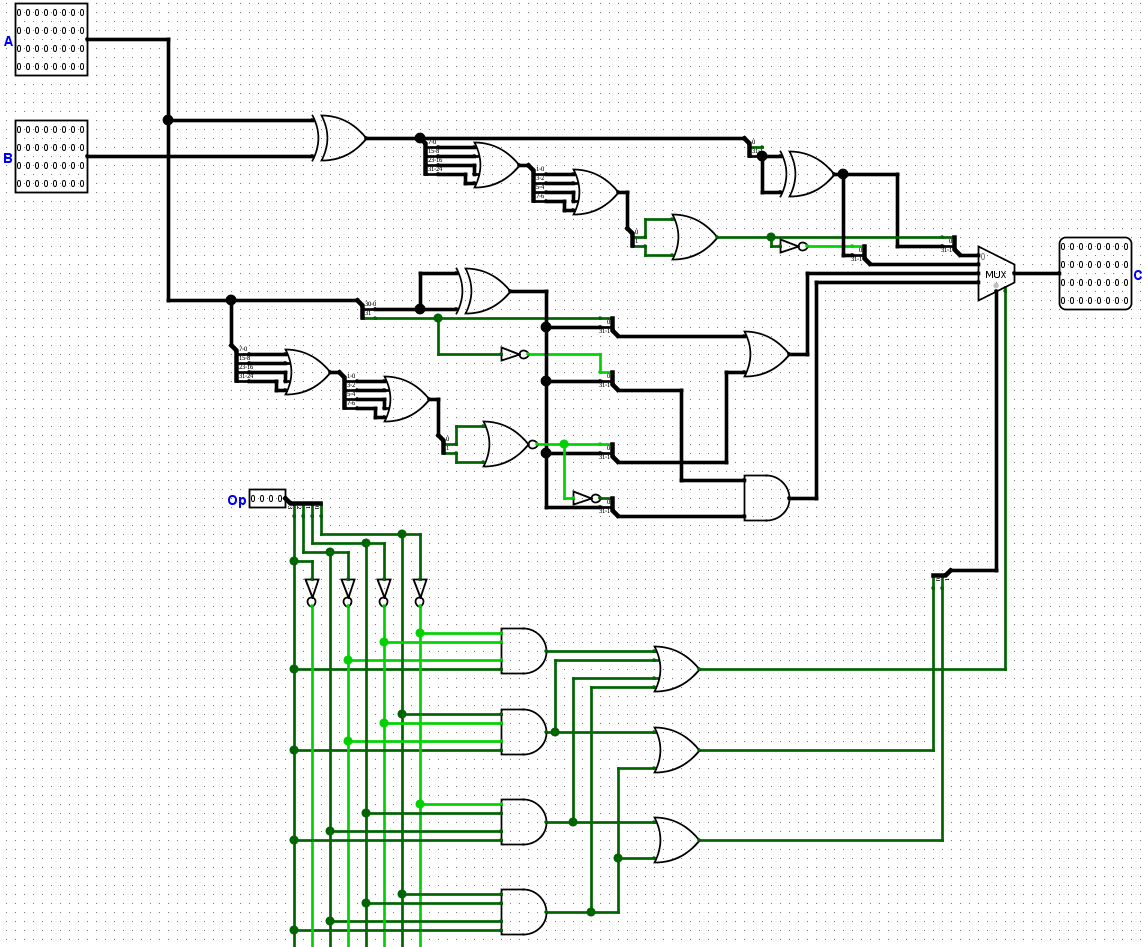
\includegraphics[width=1\textwidth]{images/Comparator32.png}
\end{center}
\captionof{figure}{First version of comparator 32bit}

\hspace*{2em}This is the first version of my comparator. It's clear that it is too complex to understand and follow, so I have broken it down into smaller subcomponents as mentioned above.
\subsection{Is equal 0}
\begin{center}
    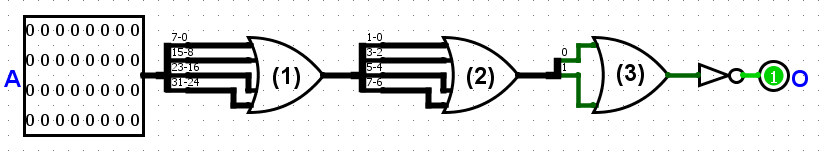
\includegraphics[width=1\textwidth]{images/IsEqual0.png}
\end{center}
\captionof{figure}{Check whether input is equal 0 or not}

\hspace{2em}To check whether the input is zero, we split the 32-bit input into 4 parts and pass each part through an OR gate. The first OR gate processes 8 bits, and if all the bits are 0, the output will be 0. If any input bit is non-zero, the output will have at least one 1. Next, we pass the 8-bit output through another OR gate, splitting it into 4 parts. This second OR gate processes 2 bits at a time, and if all inputs are 0, the output will be 0. If any bit is non-zero, at least one bit in the output will be 1. The final OR gate combines the outputs of the first and second OR gates, and if the result is 0, the output will be 0; otherwise, the output will be 1. Finally, the output passes through a NOT gate: if the value is 0, the output is 1; if the value is non-zero, the output is 0.

\hspace{2em}The first OR gate with label 1 got 8 gates count since it is 8 data bits gate. The second OR gate with label 2 got 2 gates count since it is 2 data bits gate. Then the total gates count of this block is 8 + 2 + 1 = 12 gate counts

\hspace{2em}This critical path of this block is 3
\subsection{Is equal}
\begin{center}
    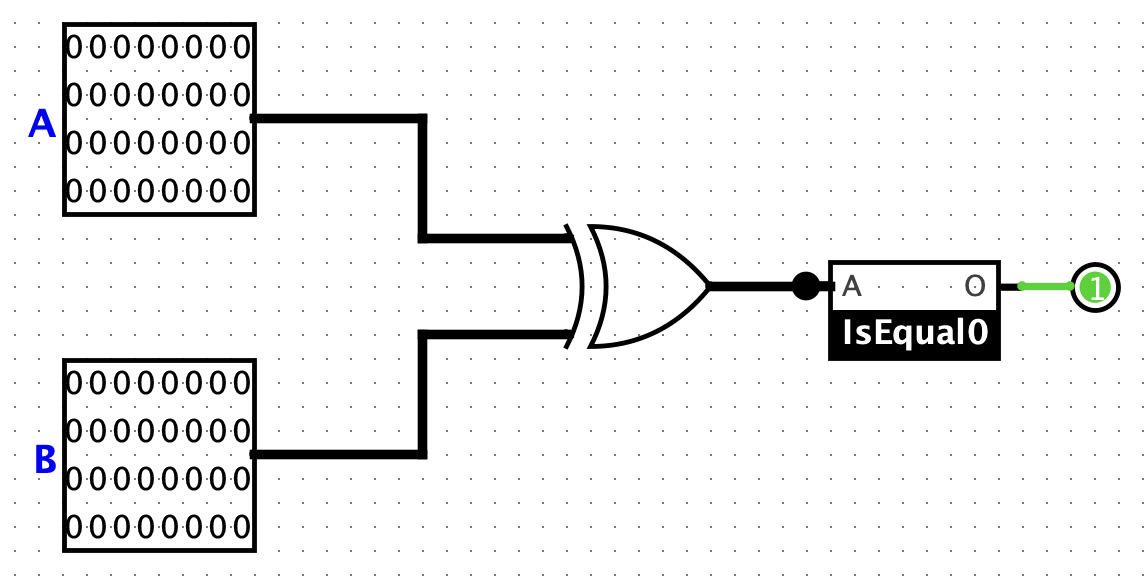
\includegraphics[width=1\textwidth]{images/IsEqual.png}
\end{center}
\captionof{figure}{Check whether A and B is equal or not}

\hspace{2em} A key property of XOR is that any number XORed with itself results in 0 (\( A \oplus A = 0 \)). To compare two numbers, we XOR them. If the result is 0, the numbers are equal; otherwise, they are not equal. To finalize the comparison, we check whether the XOR result is 0 using a "zero check" mechanism. The output is 1 if the numbers are equal and 0 if they are not.

\hspace{2em}The first xor gate got 32 gates count since it is 32 data bit gate. The is equal 0 block got 12 gates counts. Then the total gate counts of this block is 32 + 12 = 44 gates counts.

\hspace{2em}The critical path of this block is 3 + 1 = 4
\subsection{Bit extend 1 to 32bits}
\begin{center}
    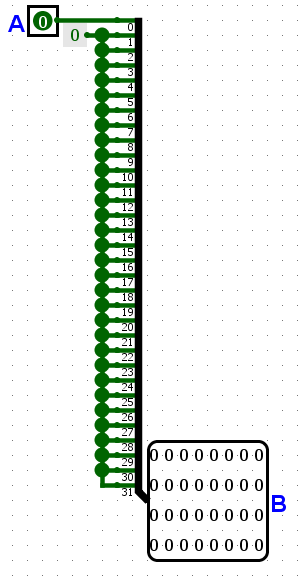
\includegraphics[width=0.5\textwidth]{images/BitExtend1to32.png}
\end{center}
\captionof{figure}{Extend 1bit input to 32bit using zero extension}

\hspace*{2em}To create a 32-bit bit extender, we use a 1-bit input as the least significant bit (LSB) of the output, while all other bits of the output are set to 0

\hspace{2em}This block got 0 gate counts

\hspace{2em}The critical path of this block is 0
\subsection{Less than or equal to 0}
\begin{center}
    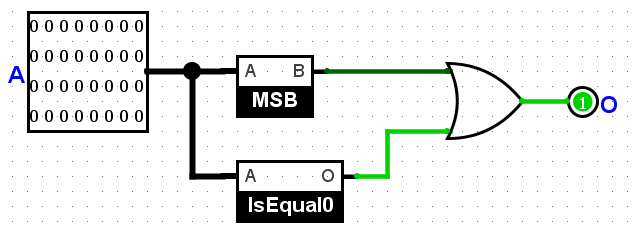
\includegraphics[width=1\textwidth]{images/LessThanOrEqual0.png}
\end{center}
\captionof{figure}{Check whether input is less than or equal 0 or not}

\hspace{2em}To check whether the input is less than or equal to 0, we combine two components using an OR gate. The first component is an "is equal to 0" circuit, and the second is a "most significant bit" (MSB) extractor circuit. In two's complement representation, if the MSB is 1, the number is negative. The outputs of these two components are ORed together to produce the final result.

\hspace{2em}This block got 12 (from the is equal 0) + 1 = 13 gates counts

\hspace{2em}The critical path of this block is 3
\subsection{Greater than 0}
\begin{center}
    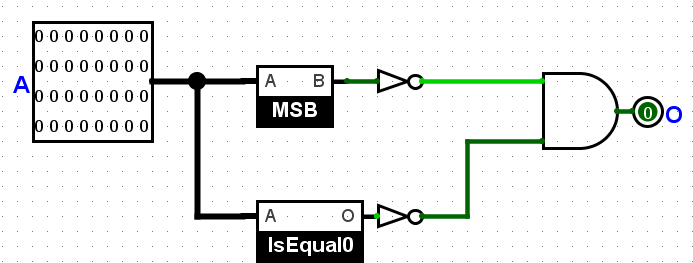
\includegraphics[width=1\textwidth]{images/GreaterThan0.png}
\end{center}
\captionof{figure}{Check whether input is greater than 0 or not}
\hspace{2em}The "check greater than 0" block operates as the opposite of the "less than or equal to 0" block. It negates the outputs of the MSB and the "is equal to 0" circuits. When the MSB is 0, the number is either 0 or positive in two's complement representation. By ANDing this with the negated result of the "is equal to 0" block, the final output will indicate whether the input is strictly greater than 0.

\hspace{2em}This block got 12 (from the is equal 0) + 1 = 13 gates counts

\hspace{2em}The critical path of this block is 3
\subsection{Operation bits}
\begin{center}
    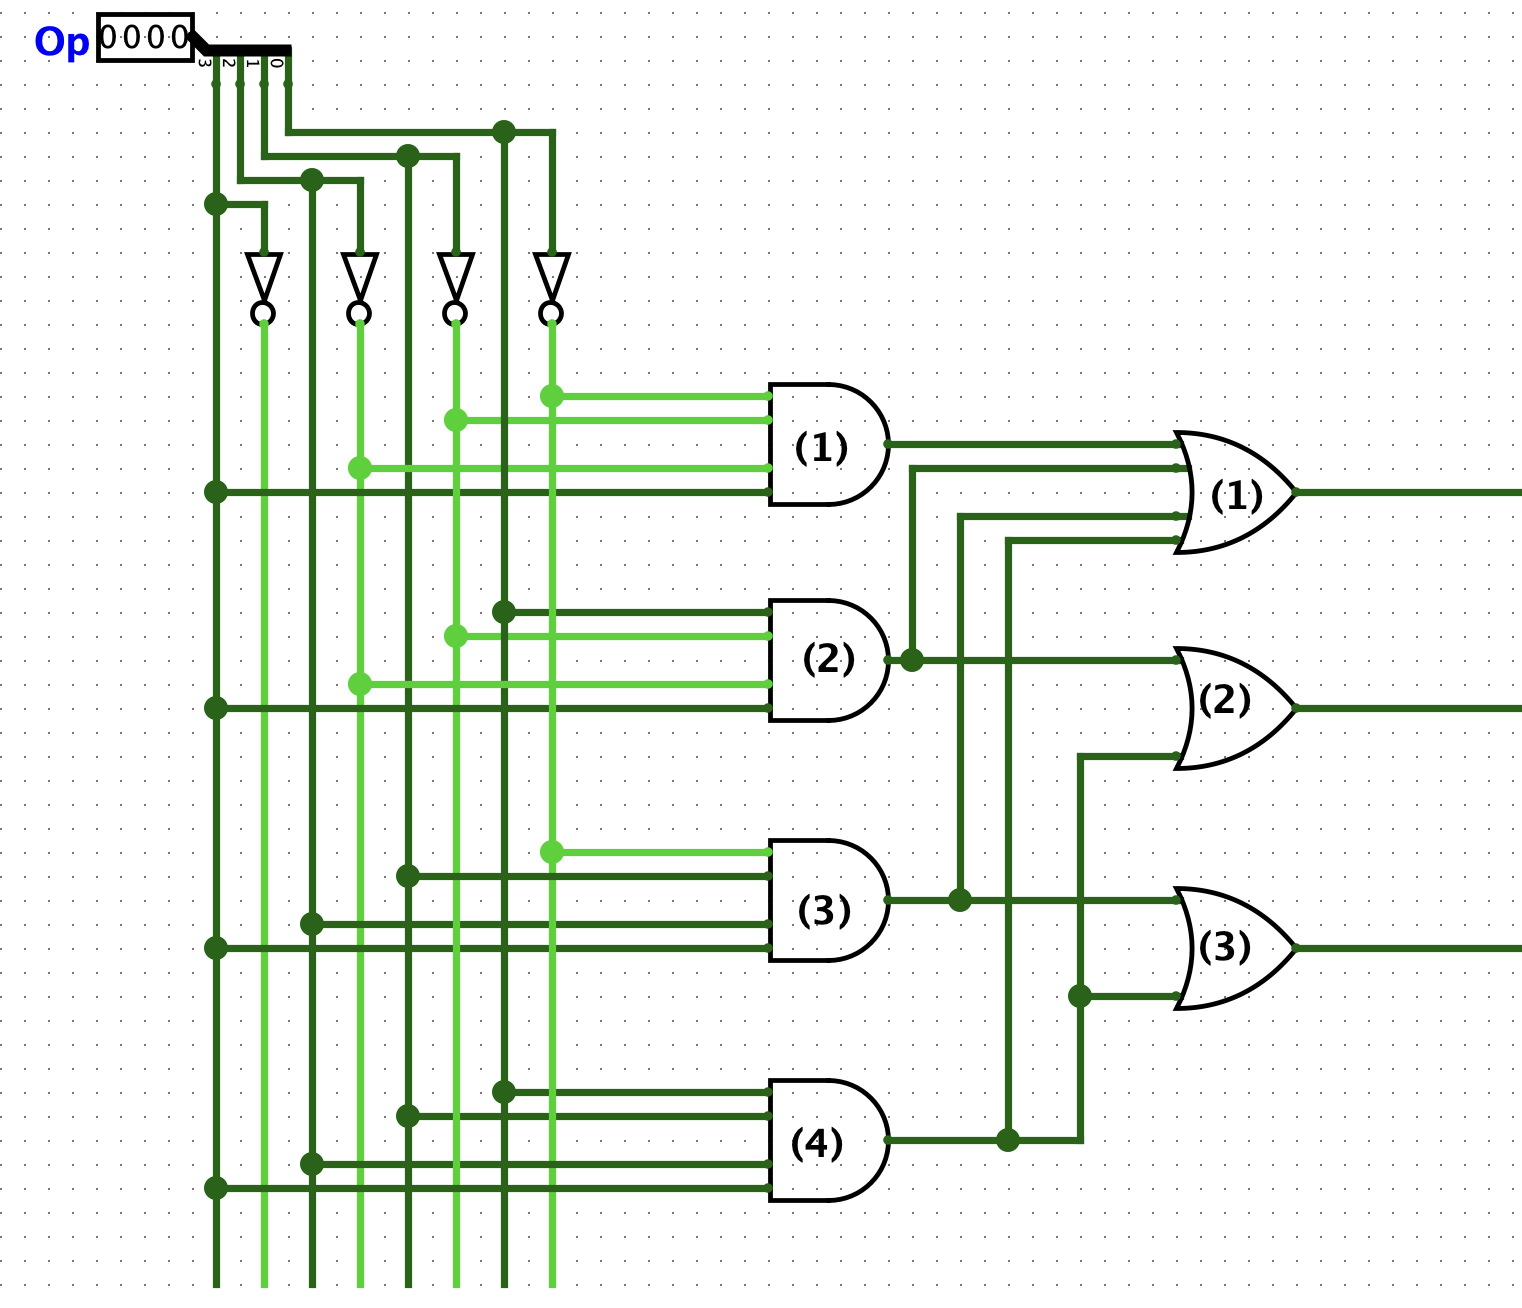
\includegraphics[width=1\textwidth]{images/ComparatorSelectionBits.png}
\end{center}
\captionof{figure}{Comparator block operation bits}
\hspace{2em} To design this operation bit circuit, we start by creating a truth table. From the truth table, we derive the Boolean equation using minterms and express it in the sum-of-products form.

\hspace{2em} This part got 7 gate counts
\subsubsection{Truth table}
\begin{table}[H]
\centering
\begin{tabular}{|c|c|c|c|c|c|c|c|c|}
\hline
Name & Op & Op3 & Op2 & Op1 & Op0 & Enable bit & Output 1 & Output 0 \\ \hline
not equal & 1000 & 1 & 0 & 0 & 0 & 1 & 0 & 0 \\ \hline
equal & 1001 & 1 & 0 & 0 & 1 & 1 & 0 & 1 \\ \hline
less than or equal 0 & 1110 & 1 & 1 & 1 & 0 & 1 & 1 & 0 \\ \hline
greater than 0 & 1111 & 1 & 1 & 1 & 1 & 1 & 1 & 1 \\ \hline
\end{tabular}
\end{table}
\subsubsection{Boolean equations}
The Boolean equations for the circuit are as follows:

\[
\text{Output}_0 = \text{Op}_3 \cdot \text{Op}_2' \cdot \text{Op}_1' \cdot \text{Op}_0 + \text{Op}_3 \cdot \text{Op}_2 \cdot \text{Op}_1 \cdot \text{Op}_0
\]

\[
\text{Output}_1 = \text{Op}_3 \cdot \text{Op}_2 \cdot \text{Op}_1 \cdot \text{Op}_0' + \text{Op}_3 \cdot \text{Op}_2 \cdot \text{Op}_1 \cdot \text{Op}_0
\]

\[
\text{EnableBit} = \text{Op}_3 \cdot \text{Op}_2' \cdot \text{Op}_1' \cdot \text{Op}_0' + \text{Op}_3 \cdot \text{Op}_2' \cdot \text{Op}_1' \cdot \text{Op}_0 + \text{Op}_3 \cdot \text{Op}_2 \cdot \text{Op}_1 \cdot \text{Op}_0' + \text{Op}_3 \cdot \text{Op}_2 \cdot \text{Op}_1 \cdot \text{Op}_0
\]

The output is a 2-bit value defined by two bits:

The least significant bit is OR-ed together (the OR label 2) by two AND terms: 

\[
\text{Op}_3 \cdot \text{Op}_2' \cdot \text{Op}_1' \cdot \text{Op}_0 \quad (\text{AND label 2})
\]

and 

\[
\text{Op}_3 \cdot \text{Op}_2 \cdot \text{Op}_1 \cdot \text{Op}_0 \quad (\text{AND label 4}).
\]

The most significant bit is OR-ed together (the OR label 3) by two AND terms: 

\[
\text{Op}_3 \cdot \text{Op}_2 \cdot \text{Op}_1 \cdot \text{Op}_0' \quad (\text{AND label 3})
\]

and the AND label 4.

The output will identify which comparator to select:
\[
\begin{array}{l}
00 \text{ for not equal} \\
01 \text{ for equal} \\
10 \text{ for less than or equal 0} \\
11 \text{ for greater than 0}
\end{array}
\]

The enable bit will be OR-ed (the OR label 1) by the AND label 4, and the AND labels 2, 3, 4, and \(\text{Op}_3 \cdot \text{Op}_2' \cdot \text{Op}_1' \cdot \text{Op}_0' \quad (\text{AND label 1})\). This will be used for the input of the enable bit of the MUX; if not, the result of this block will be zero.


\subsection{Comparator Block}
\begin{center}
    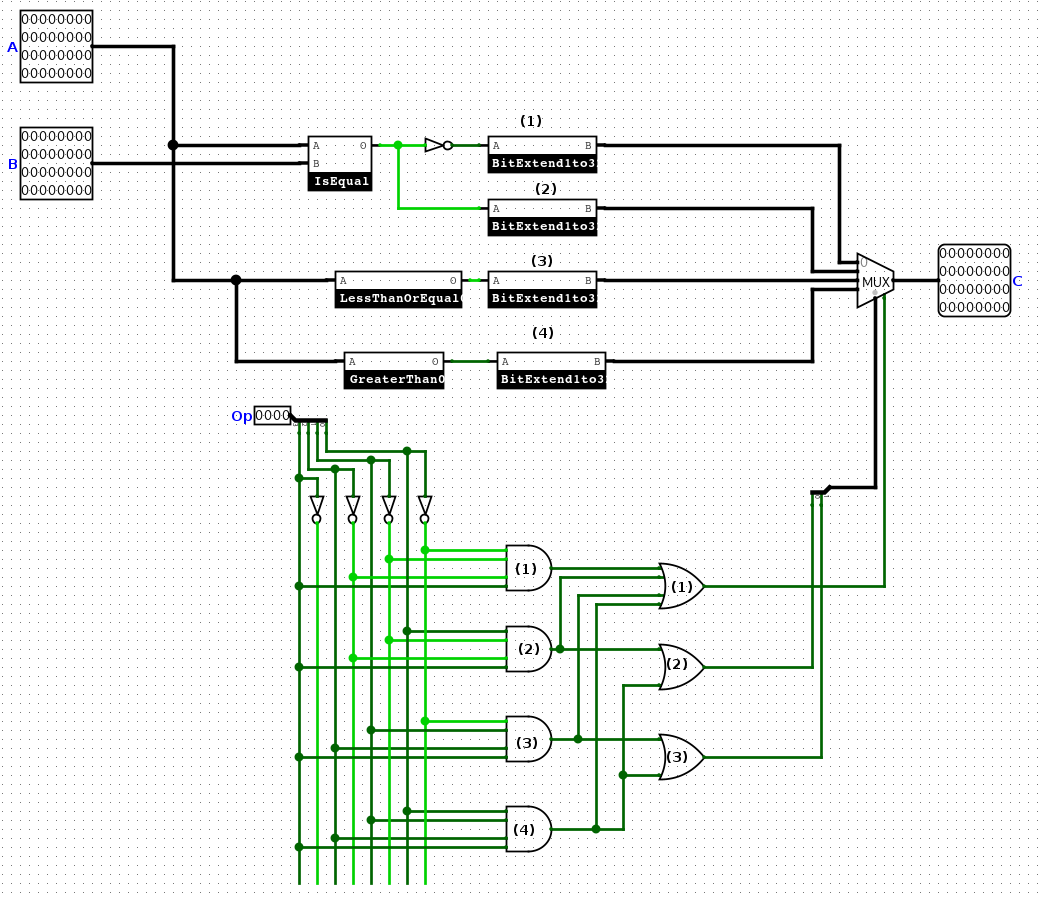
\includegraphics[width=1\textwidth]{images/Comparator32Upgraded.png}
\end{center}
\captionof{figure}{Final version of comparator block}
\noindent The 32-bit comparator block utilizes all the components in this section. It consists of four 1-to-32 bit extend blocks, each connected to the input of a 4-to-1 multiplexer to select the correct result:

\begin{enumerate}
    \item \textbf{First Bit Extend Block (Not Equal Check):}  
    The first bit extend block is connected to the not of "is equal" comparator, which checks whether the values are not equal.
    
    \item \textbf{Second Bit Extend Block (Equal Check):}  
    The second bit extend block is connected to the "is equal" comparator, which checks whether the values are equal.
    
    \item \textbf{Third Bit Extend Block (Less Than or Equal to 0 Check):}  
    The third bit extend block checks whether input \( B \) is less than or equal to 0.
    
    \item \textbf{Fourth Bit Extend Block (Greater Than 0 Check):}  
    The fourth bit extend block checks whether input \( B \) is greater than 0.
\end{enumerate}

\noindent These four results are then passed into a 4-to-1 multiplexer, which selects the correct output based on the operation. The multiplexer also receives an enable signal from the ORed result of label 1:
\begin{itemize}
    \item If the enable bit is \( 0 \), the output will be a 32-bit value of \( 0 \).
\end{itemize}


\hspace{2em}The 4-to-1 mux got 32 * (4 + 1)= 160 gates counts. The block is equal got 44 gates coounts. The block less than or equal 0 and greater than 0 each got 12 gates counts. The total gates counts of this block is 160 + 44 + 12 * 2 + 7 = 235 gates counts.

\hspace{2em}The critical path of this block is 2 + 3 = 5

\section{Logical 32bit}
\hspace*{2em}The logical block is the simplest component to create. We can directly use standard logic gates and adjust the data width from 1 bit to 32 bits to match the desired result.
\subsection{Operation bits}
\hspace{2em} To design this operation bit circuit, we start by creating a truth table. From the truth table, we derive the Boolean equation using minterms and express it in the sum-of-products form.
\begin{center}
    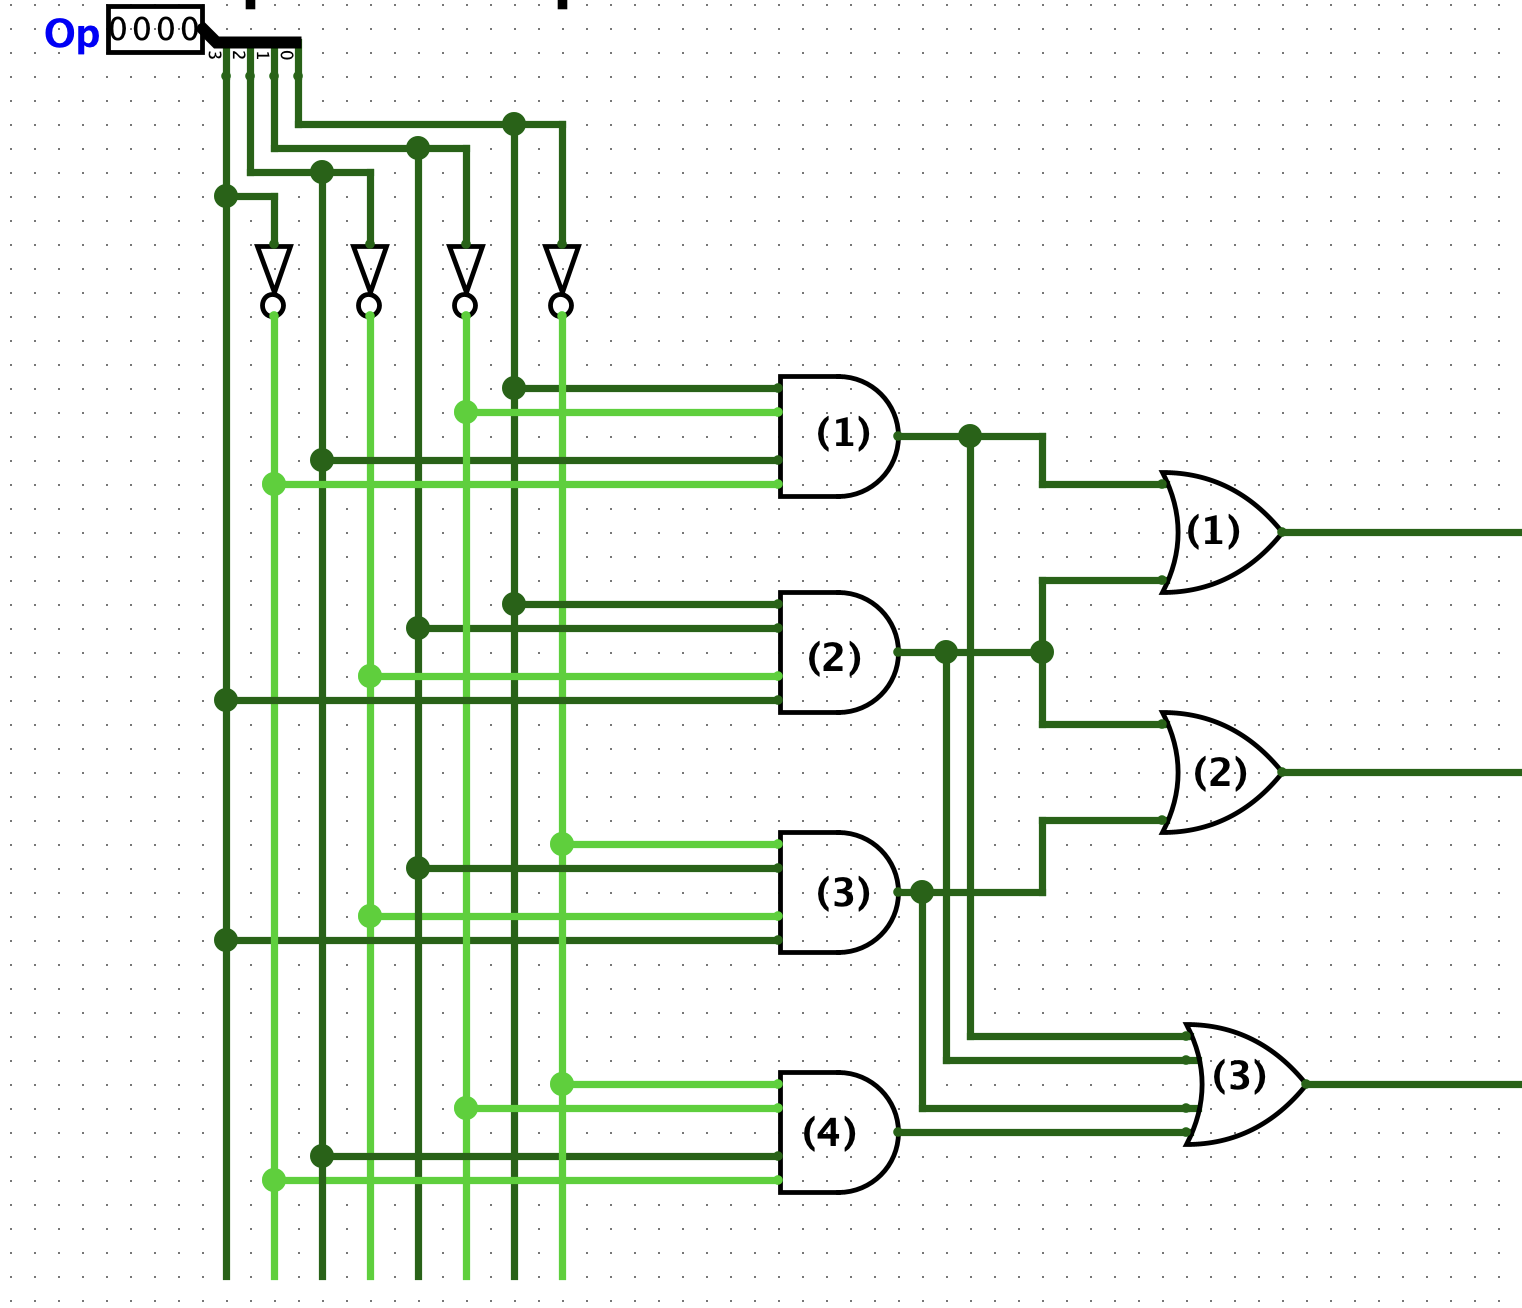
\includegraphics[width=1\textwidth]{images/LogicalSelectionBits.png}
\end{center}
\captionof{figure}{Logical block operation bits}

\hspace{2em} This part got total 7 gate counts

\subsubsection{Truth table}
\begin{table}[H]
\centering
\begin{tabular}{|c|c|c|c|c|c|c|c|c|}
\hline
Name & Op & Op3 & Op2 & Op1 & Op0 & Enable bit & Output 1 & Output 0 \\ \hline
and & 0100 & 0 & 1 & 0 & 0 & 1 & 0 & 0 \\ \hline
or & 0101 & 0 & 1 & 0 & 1 & 1 & 0 & 1 \\ \hline
xor & 1010 & 1 & 0 & 1 & 0 & 1 & 1 & 0 \\ \hline
nor & 1011 & 1 & 0 & 1 & 1 & 1 & 1 & 1 \\ \hline
\end{tabular}
\end{table}

\subsubsection{Boolean equations}
The Boolean equations for the circuit are as follows:

\[
\text{Output}_0 = \text{Op}_3' \cdot \text{Op}_2 \cdot \text{Op}_1' \cdot \text{Op}_0 + \text{Op}_3 \cdot \text{Op}_2' \cdot \text{Op}_1 \cdot \text{Op}_0
\]

\[
\text{Output}_1 = \text{Op}_3 \cdot \text{Op}_2' \cdot \text{Op}_1 \cdot \text{Op}_0' + \text{Op}_3 \cdot \text{Op}_2' \cdot \text{Op}_1 \cdot \text{Op}_0
\]

\[
\text{EnableBit} = \text{Op}_3 \cdot \text{Op}_2' \cdot \text{Op}_1 \cdot \text{Op}_0 + \text{Op}_3' \cdot \text{Op}_2 \cdot \text{Op}_1' \cdot \text{Op}_0 + \text{Op}_3 \cdot \text{Op}_2' \cdot \text{Op}_1 \cdot \text{Op}_0' + \text{Op}_3 \cdot \text{Op}_2' \cdot \text{Op}_1 \cdot \text{Op}_0
\]

The output is a 2-bit value defined by two bits:

The least significant bit is OR-ed together (the OR label 1) by two AND terms:

\[
\text{Op}_3' \cdot \text{Op}_2 \cdot \text{Op}_1' \cdot \text{Op}_0 \quad (\text{AND label 1})
\]

and

\[
\text{Op}_3 \cdot \text{Op}_2' \cdot \text{Op}_1 \cdot \text{Op}_0 \quad (\text{AND label 2}).
\]

The most significant bit is OR-ed together (the OR label 2) by two AND terms:

\[
\text{Op}_3 \cdot \text{Op}_2' \cdot \text{Op}_1 \cdot \text{Op}_0' \quad (\text{AND label 3})
\]

and the AND label 2.

The output will identify which comparator to select:

\[
\begin{array}{l}
00 \text{ for AND} \\
01 \text{ for OR} \\
10 \text{ for XOR} \\
11 \text{ for NOR}
\end{array}
\]

The enable bit will be OR-ed (the OR label 3) by the AND label 4, and the AND labels 1, 2, 3, and \(\text{Op}_3 \cdot \text{Op}_2' \cdot \text{Op}_1 \cdot \text{Op}_0 \quad (\text{AND label 4})\). This will be used for the input of the enable bit of the MUX; if not, the result of this block will be zero.


\subsection{Logical Block}
\begin{center}
    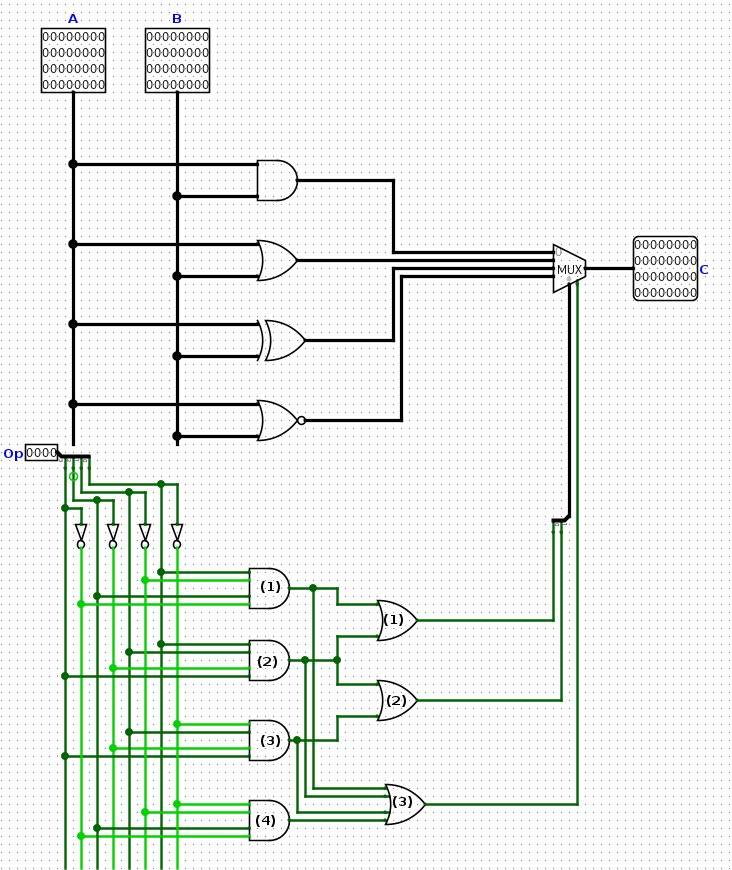
\includegraphics[width=1\textwidth]{images/Logical32.png}
\end{center}
\captionof{figure}{Final version of logical block}
\begin{enumerate}
    \item \textbf{Logic Gate Operations:}  
    \begin{itemize}
        \item The input data is processed through four logic gates: AND, OR, XOR, and NOR.
        \item Each gate receives two 32-bit input values.
    \end{itemize}

    \item \textbf{Multiplexer Selection:}  
    \begin{itemize}
        \item The outputs of the four logic gates are passed through a 4-to-1 multiplexer.
        \item The multiplexer selects the result of the desired operation based on the control signal.
    \end{itemize}

    \item \textbf{Enable Bit Control:}  
    \begin{itemize}
        \item The multiplexer also uses an enable bit to determine whether to output the result of this block.
        \item If the block is not enabled, the output is a 32-bit value of \( 0 \).
    \end{itemize}
\end{enumerate}

\hspace{2em}Each AND, OR, XOR, and NOR gates got 32 gates count since each is 32 data bit gate. The 4-to-1 mux got 32 ( 4 + 1) = 160 gate counts. Then the total gate count of this block is 32 * 4 + 160 + 7 = 295 gates counts

\hspace{2em}The critical path of this block is 1 + 2 = 3

\section{Conclusion}
\hspace{2em}The total gate count of the $\text{ALU32}$ is calculated as follows:
\[
\begin{align*}
\text{Total Gate Count} &= 295 \, (\text{Logical Block}) + 235 \, (\text{Comparator Block}) \\
&\quad + 805 \, (\text{Shifter Block}) + 388 \, (\text{Add/Sub Block}) \\
&\quad + 32 \, (\text{OR Gates in ALU32 Circuit}) = 1755 \, \text{Gates}.
\end{align*}
\]

\hspace{2em}The critical of this ALU is the maximum path length of 4 block Add and Sub block, Shifter block, Comparator block and logical block which is 69. With the last OR of the ALU 32 the critical path of this ALU32 is 70

\hspace{2em}The test vectors and the test vector generator can be accessed from the following link:  
\texttt{\href{https://github.com/truongng201/ALU-Design}{https://github.com/truongng201/ALU-Design}}. This repository also includes an ALU (Arithmetic Logic Unit) simulator implemented in Python. The simulator operates in the same way as the ALU circuit described in this project.

\hspace{2em} Here are the successful result of 3 test vector for ALU32 block, LeftShift32 block, and Add32 block
\begin{center}
    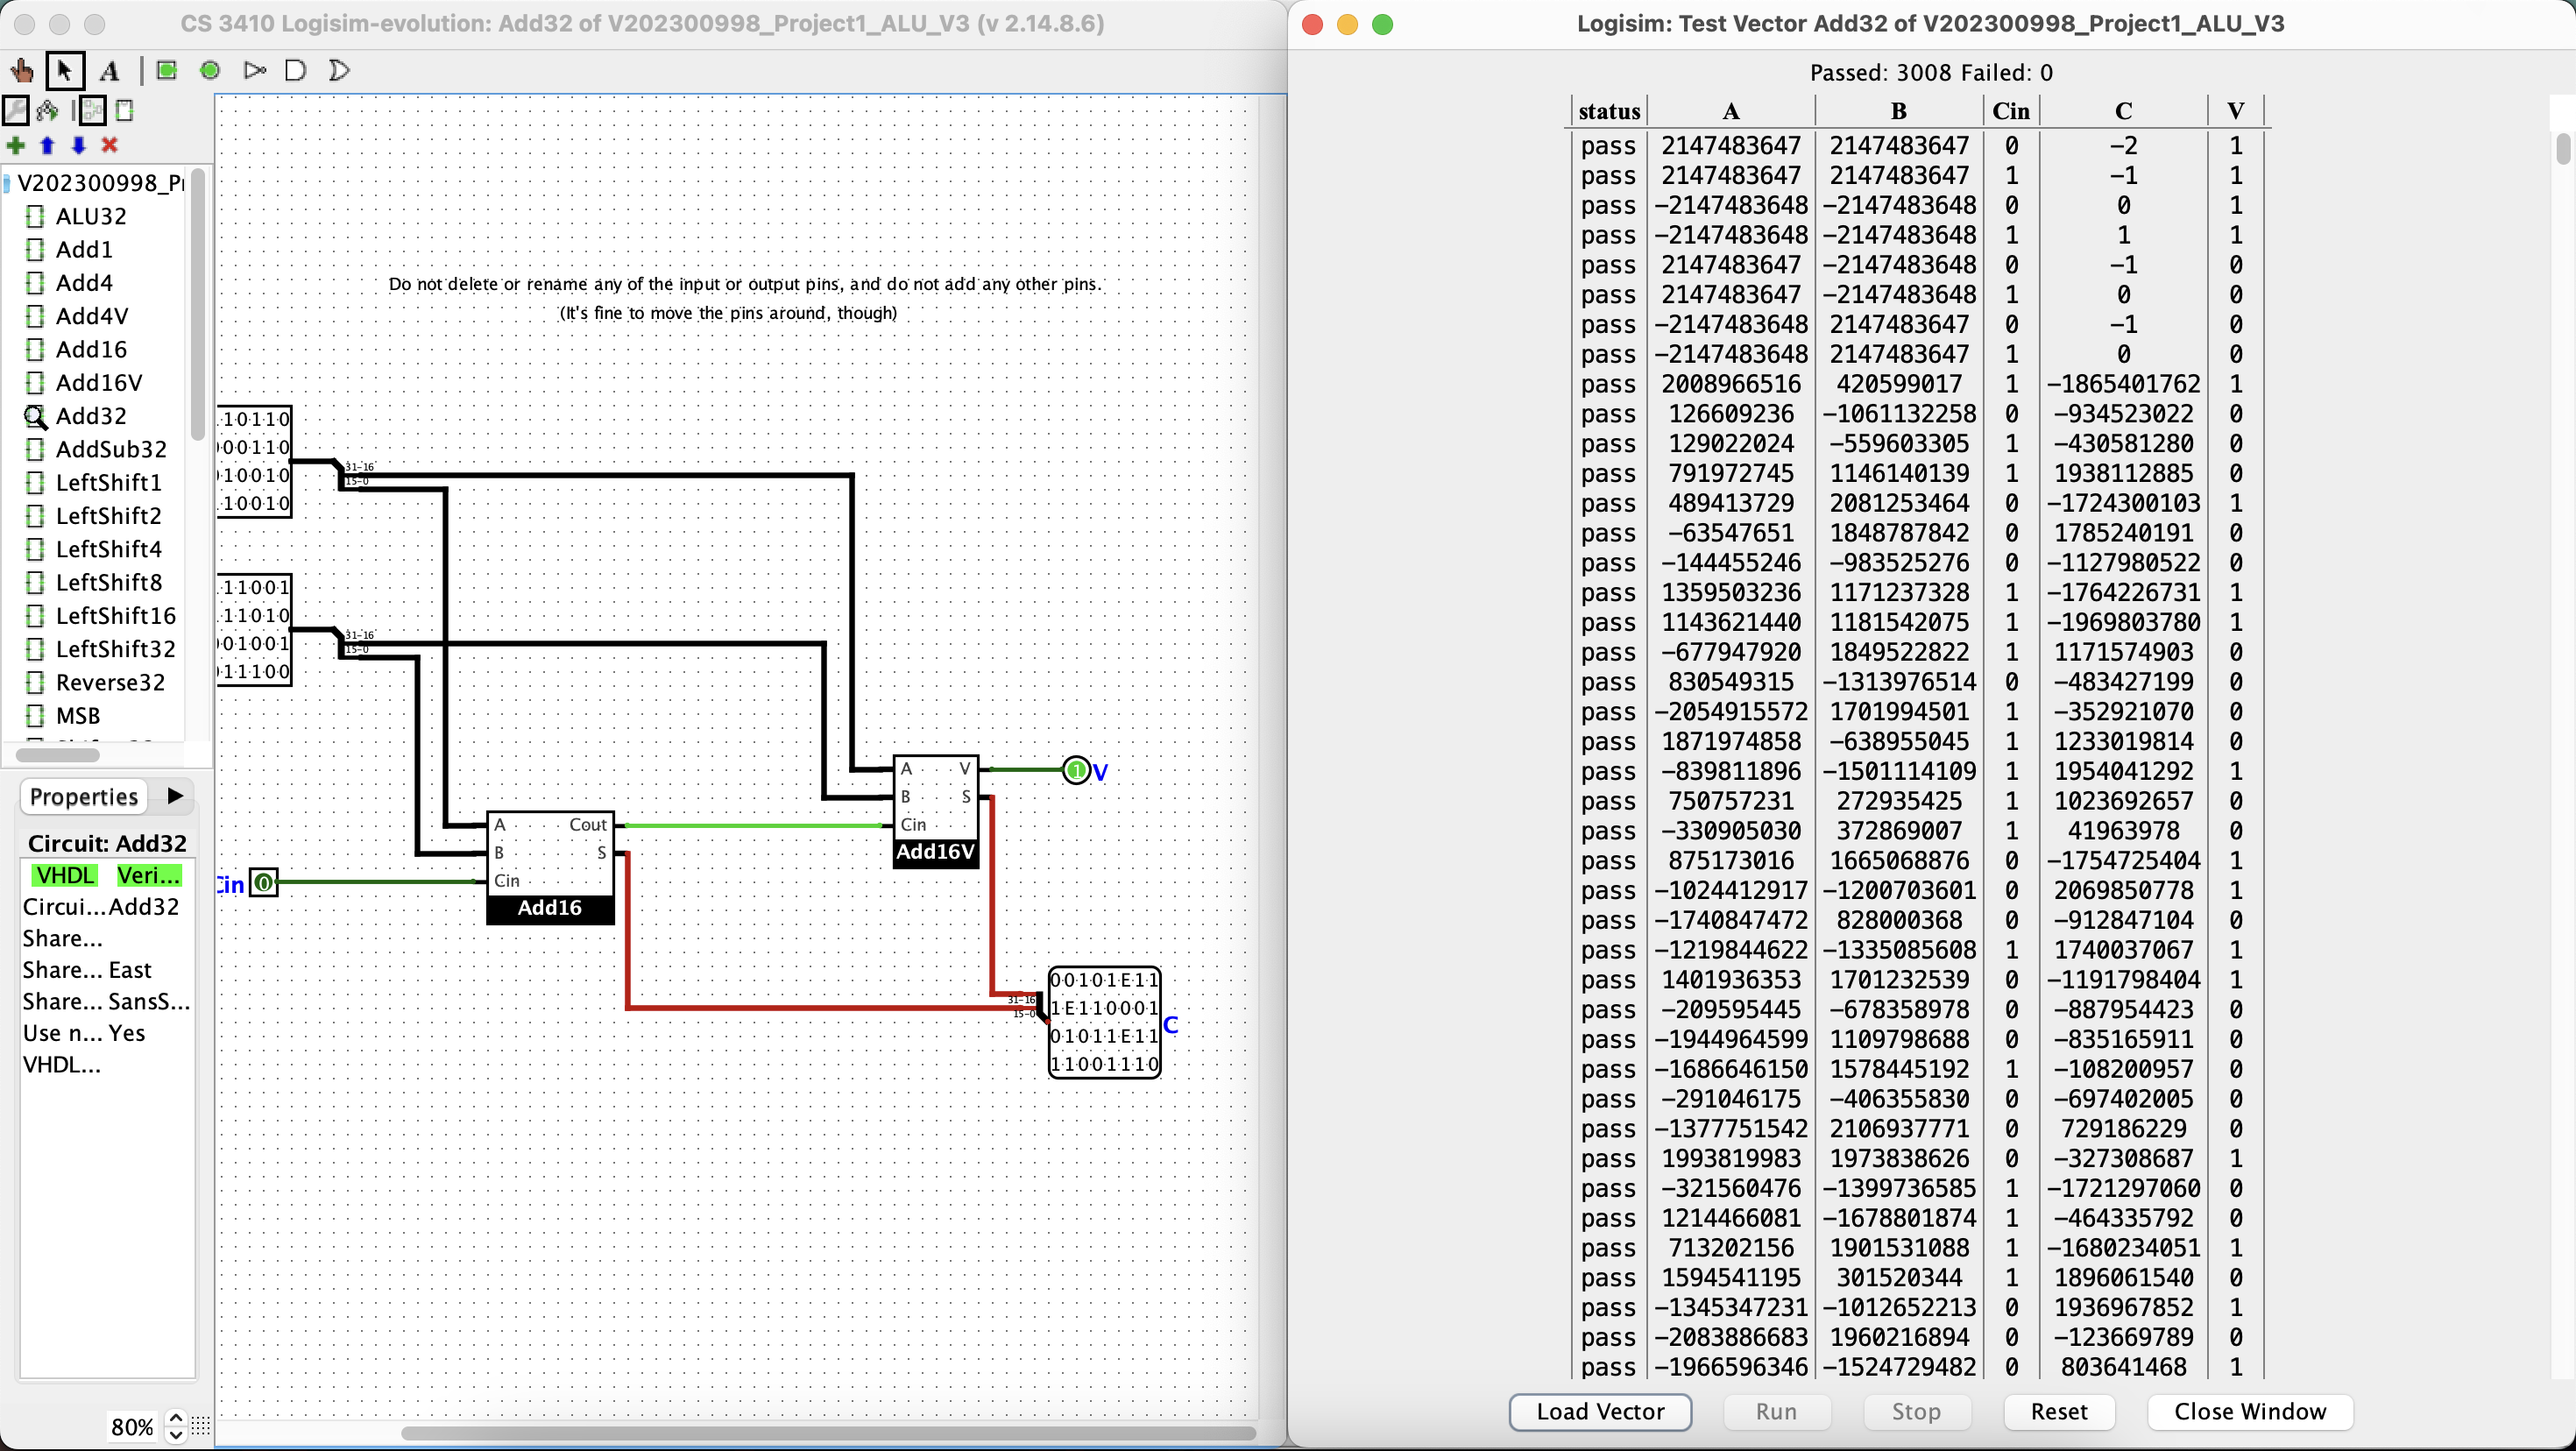
\includegraphics[width=0.8\textwidth]{images/Add_test_vector.png}
\end{center}
\begin{center}
    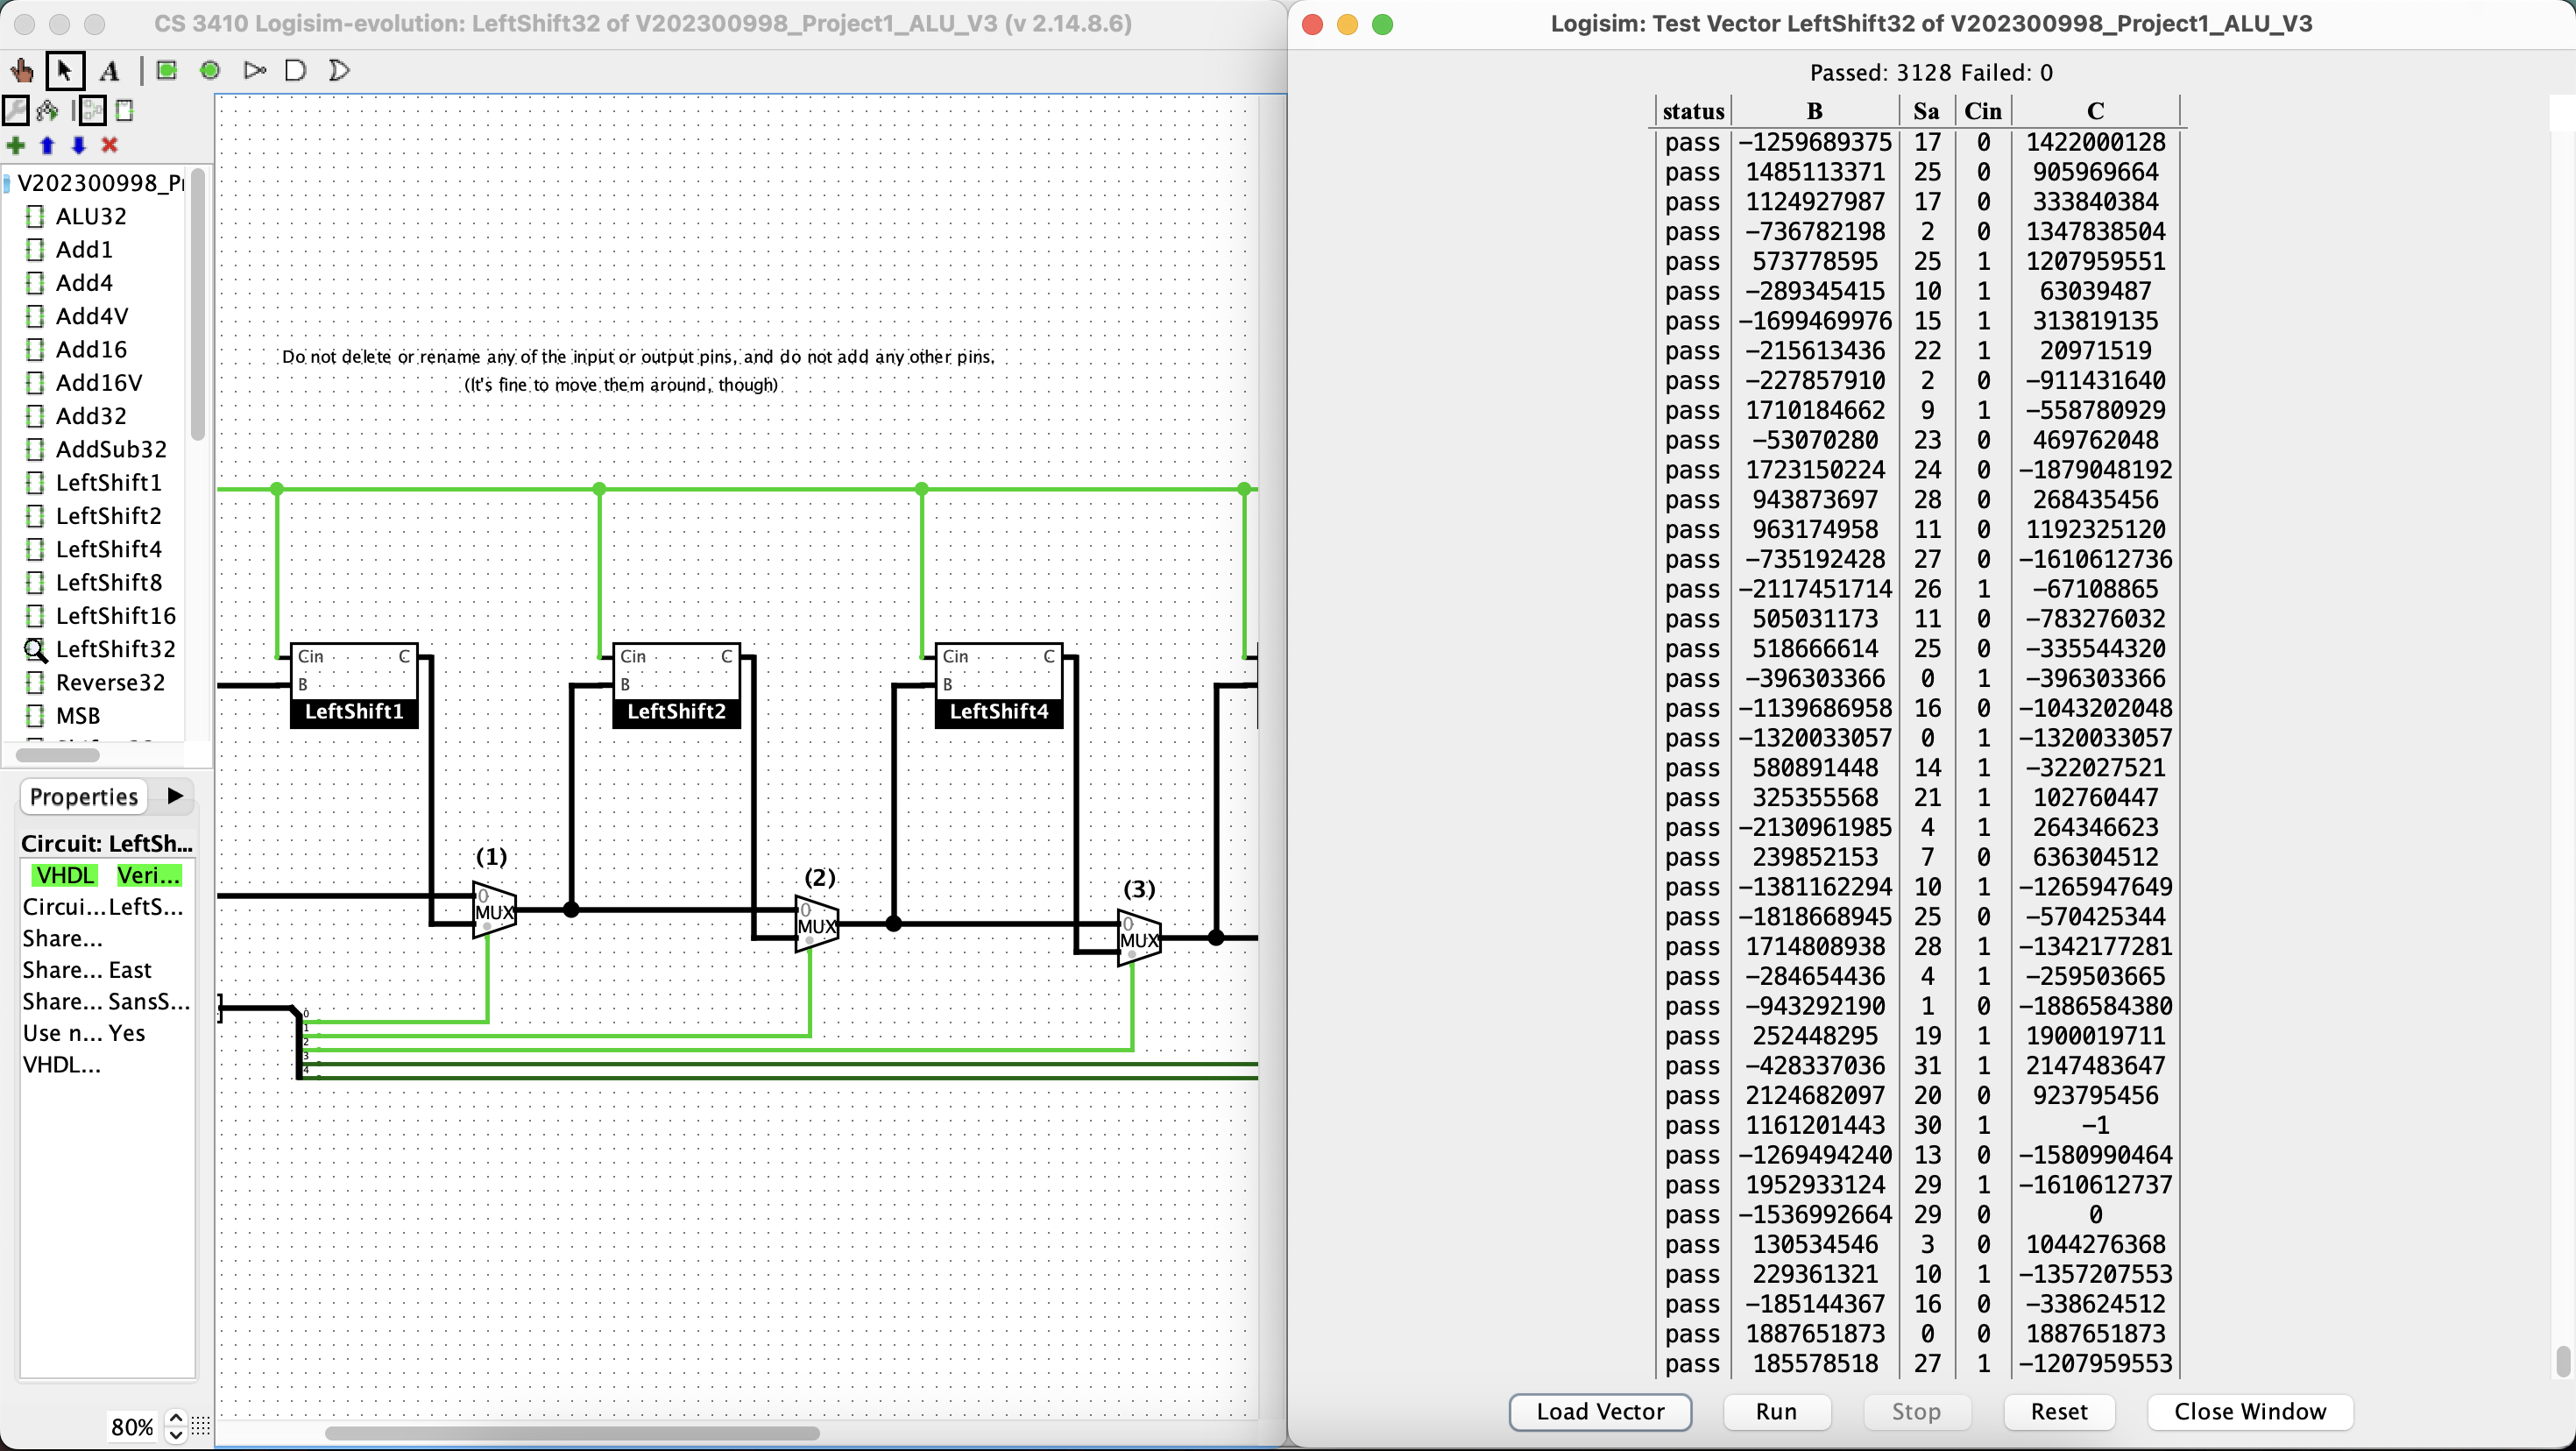
\includegraphics[width=0.8\textwidth]{images/Leftshift_test_vector.png}
\end{center}
\begin{center}
    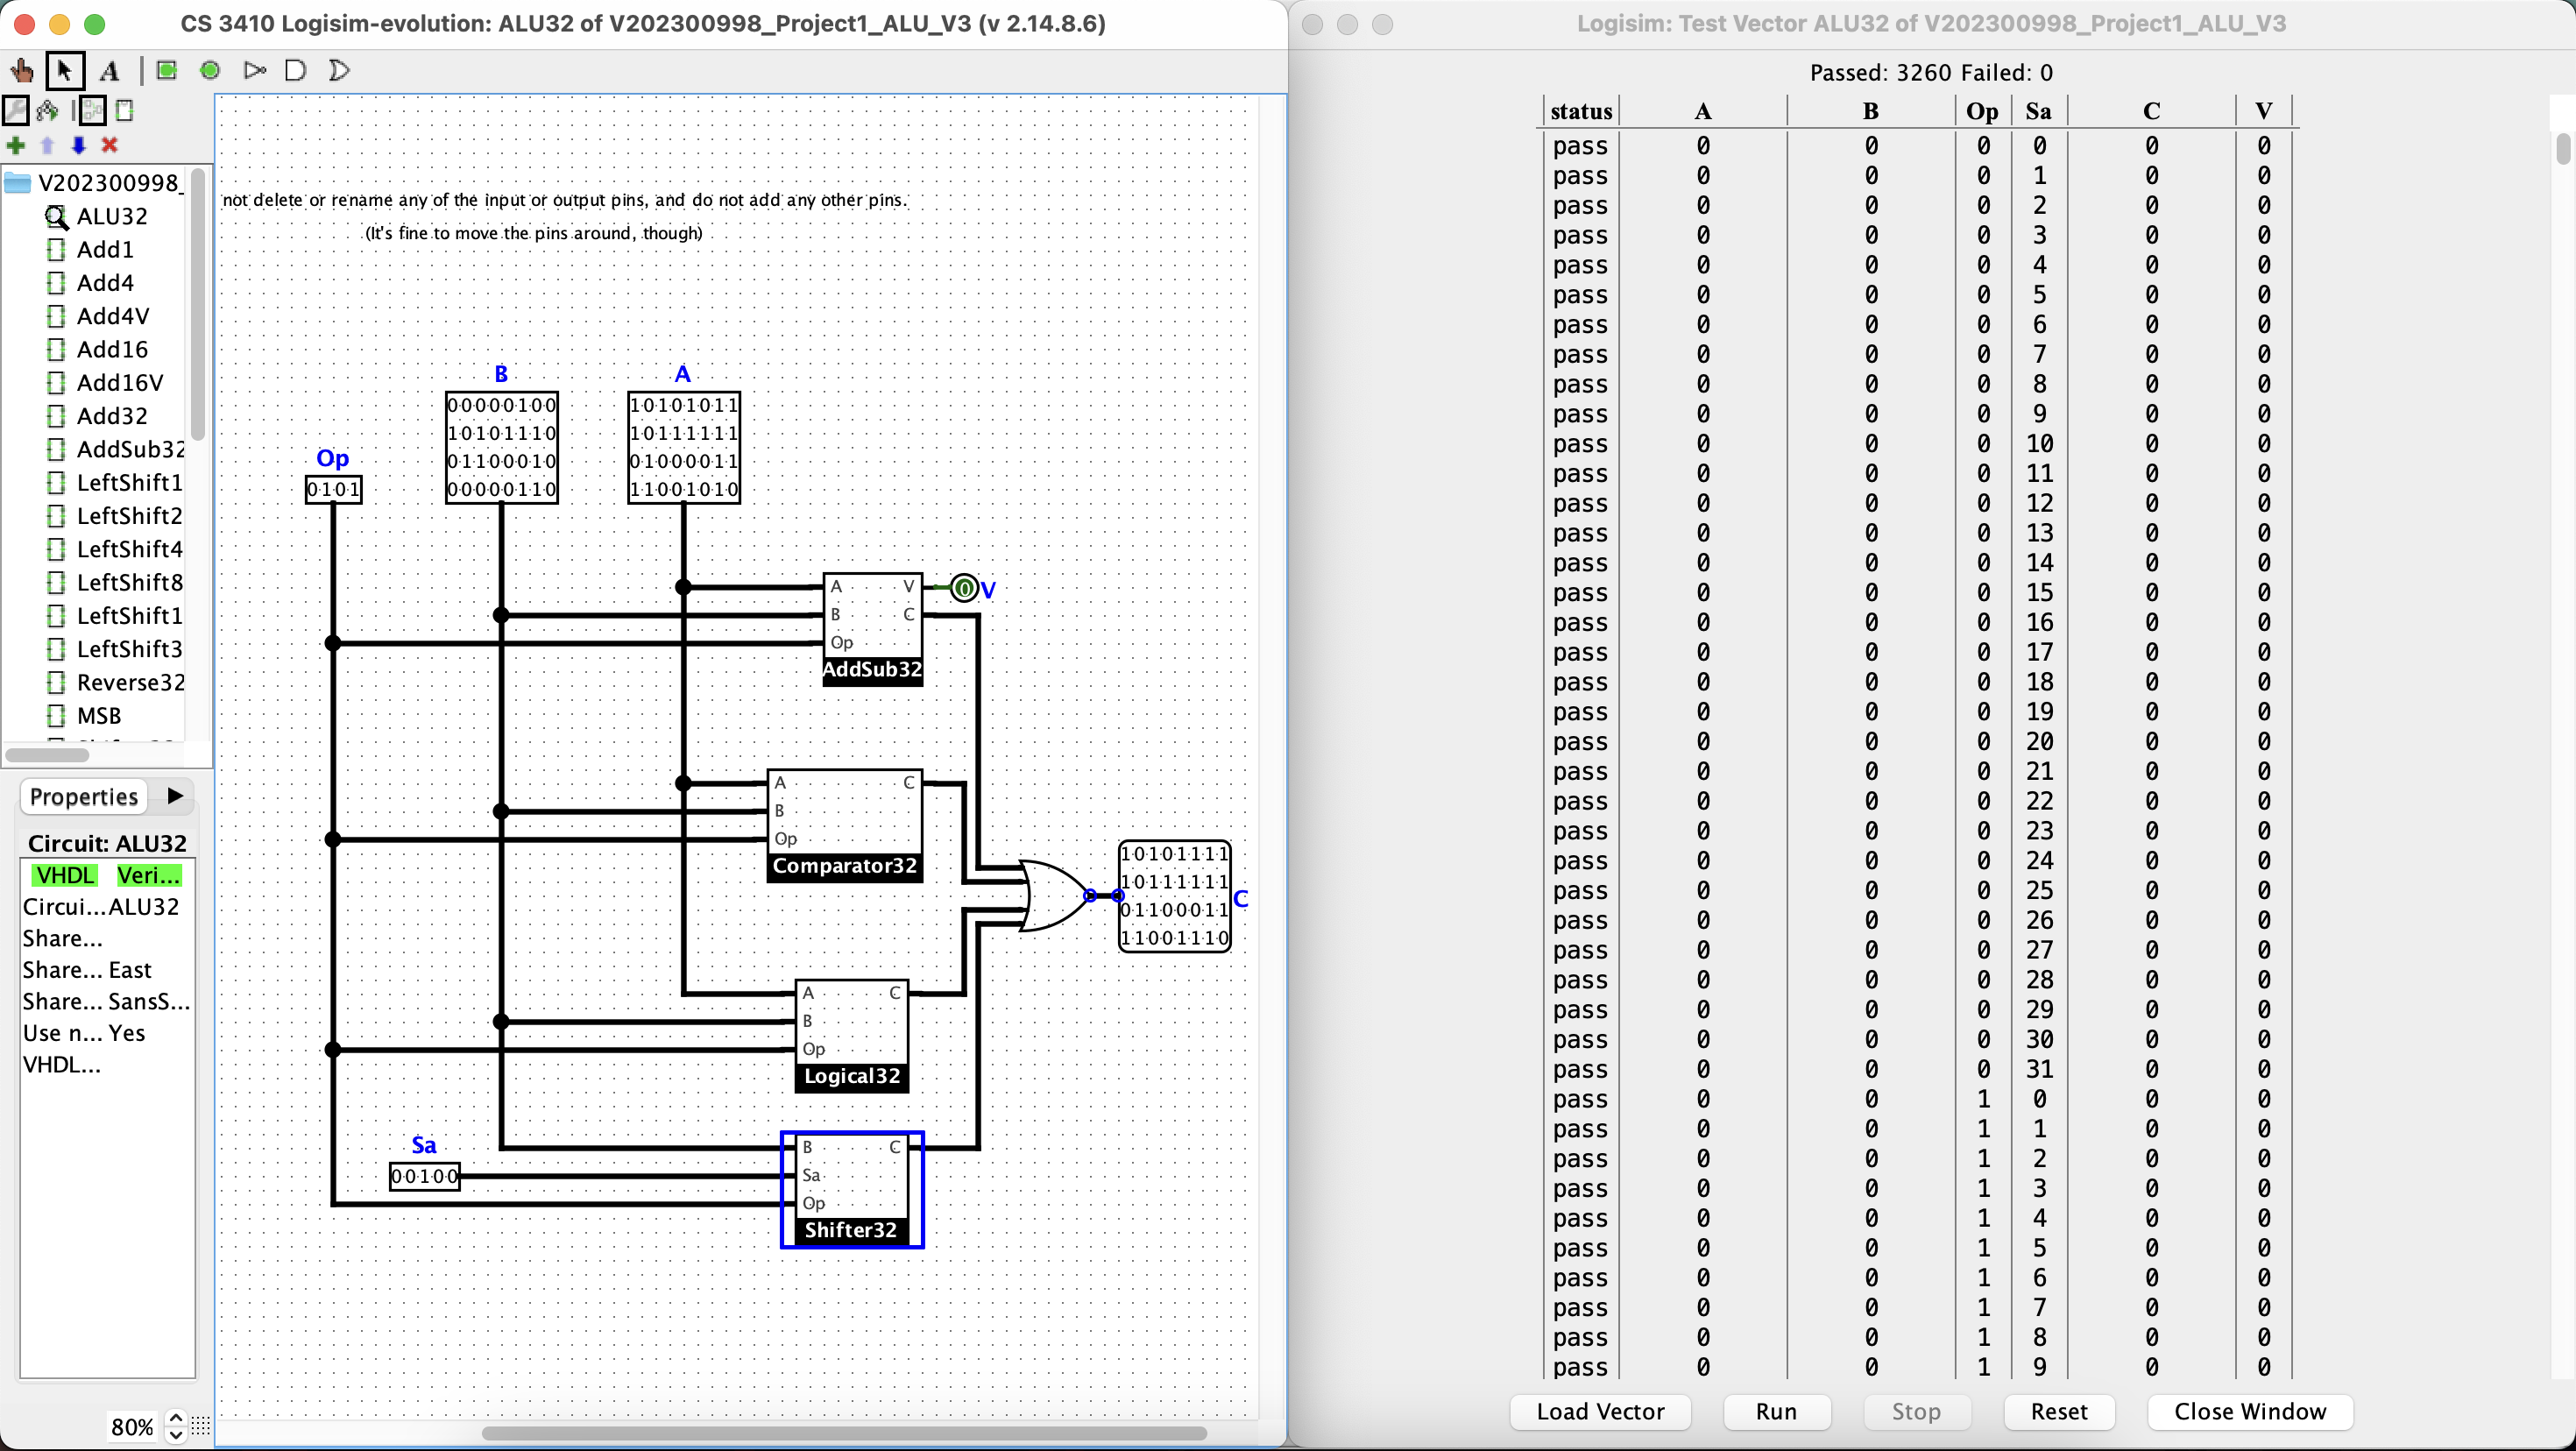
\includegraphics[width=0.8\textwidth]{images/ALU_test_vector.png}
\end{center}
\end{document}

